\chapter{Automatic workflows for aerodynamic simulations}
\label{chap4}

\section{Introduction}
\label{sec4.1}

Since the very beginning, the main purpose behind the development of a library devoted to the automatic generation of 3D \gls{CAD} models of aircrafts has been the possibility of using the same models for aerodynamic analyses, carried out by the use of a \gls{CFD} software. For this reason, the models produced by \gls{JPAD} come equipped with solutions (such as the modeling of the wing tip, or the automatic gap enhancement of the aifoils trailing edge in case of necessity) that make them ready to be imported and used into a suite for aerodynamics investigations. Moreover, since the models are generated without the necessity of human intervention during the process, and considering that the classes of \gls{JPAD} offer the possibility to make changes to the geometric characteristics of aircraft components once imported from data file, what comes to mind is the possibility to integrate the \lstinline[language=Java]!JPADCAD! module, along with the \lstinline[language=Java]!AircraftUtils! functionalities, in a comprehensive development cycle involving \gls{CFD} analyses. By use of the aforementioned functions and classes, in fact, it becomes possible to automatically produce several geometries of the same aircraft, differing in some characteristics (e.g., the wing aspect ratio, or the dihedral angle). These models should be then imported, one at a time and in an automatic way, into a software for Computational Fluid Dynamics, in order to perform on them all the necessary analyses and produce the requested results. What becomes necessary at this point is some sort of \emph{bridge}, connecting \gls{JPAD} and all its modules to some existing \gls{CFD} software. This software, however, based on what has been said above, must fulfill the following requirements:
%
\begin{itemize}
\item must provide support for recording and playing macros,
\item must give the possibility to run macros in batch mode.
\end{itemize}   
%
These macros are going to collect all the operations that will be performed by the \gls{CFD} software, from importing the \gls{CAD} models to collecting results. In this way, one can think to launch a complete workflow from a simple test class (i.e., a class containing just a main method) located in \gls{JPAD}, which manages all the operations, from establishing the type of the analysis to actually running the software and the macro. 

\bigskip
\noindent
Therefore a choice needs to be made about the \gls{CFD} software. CD-adapco STAR-CCM+ meets the characteristics listed above. In addition, STAR-CCM+ macros are written in Java, with this representing a great advantage, since \gls{JPAD} is written in Java too. In fact, in order for our Java macros to run properly and perform operations as we want, it is necessary to provide them support by means of dedicated classes and utilities. These classes not only are used by the macros, but can also be employed by the test class in \gls{JPAD} in order to define the characteristics of the simulations, as it will be clearer in the following paragraphs. 

\section{STAR-CCM+ overview}
\label{sec4.2}

STAR-CCM+ is not just a tool for \gls{CFD} analyses. More in general, it is a \gls{CAE} solution for solving multidisciplinary problems in both fluid and solid continuum mechanics, within a single integrated interface. The STAR-CCM+ environment offers all the tools required in order to execute engineering analyses. These tools allows the following operations:
%
\begin{itemize}
\item import and creation of geometries,
\item mesh generation,
\item solution of the governing equations,
\item analysis of the results,
\item automation of the simulation workflows for design exploration studies,
\item connection to other \gls{CAE} software for co-simulation analysis.
\end{itemize}
%
For what concerns geometries, STAR-CCM+ can read geometric data saved in neutral formats (such as IGES and STEP) or triangulated ones (such as STL). Besides, it also offers a built-in capability for modifying and creating \gls{CAD} geometries directly. Its 3D \gls{CAD} tool is a parametric feature-based modeler that is built upon the Parasolid kernel. Among its extensive suite of \gls{CAD} functions it includes important operations, such as Boolean actions, automatic removal of small bodies or surfaces irrelevant to simulation, and flow domain extraction. Regarding mesh operations, STAR-CCM+ provides a complete set of capabilities for both surface and volume meshing operations. Its mesh framework provides a flexible environment and, most importantly, repeatable processes. The principal features of the framework consist in allowing serial, concurrent per part, and parallel mesh generation, permitting the sequencing and re-ordering of mesh operations, and providing the capability to perform local mesh modifications. Being a \gls{CAE} software, STAR-CCM+ solves systems of equations derived from the fundamental laws of physics and spanning several different fields, from fluid to solid mechanics, passing through aeroacoustics and reacting flows. In order to solve these systems of equations, built from the chosen models and their boundary conditions, it makes use of numerical algorithms, based on finite volume and finite element methods. \cite{STARCCMUserGuide}

\section{A supporting package: \texttt{MacroExtras}}
\label{sec4.3}

\lstinline[language=Java]!MacroExtras! is the package containing all the \emph{extra} classes and utilities used by our STAR-CCM+ macros and by the test launching classes. These classes are arranged as figure \ref{fig:macroextraspackage} shows, while the tasks they fulfill can be listed as follows:
%
\begin{itemize}
\item provide support to XML writing and reading operations;
\item handle the entities and the parameters of the simulation;
\item provide enumerations in order to easily manage the entities and the parameters of the simulation.
\end{itemize}
%
The following paragraphs give a description of each of the classes that is contained in \lstinline[language=Java]!MacroExtras!, focusing on the Java classes used for accomplishing their tasks and on the eventual \gls{design:pattern} behind the way they have been written. 
%
\begin{figure}[H]
\centering
\includegraphics[scale=0.30]{Immagini/Capitolo4/macroextraspackage}
\caption{\lstinline[language=Java]!MacroExtras! package structure}
\label{fig:macroextraspackage}
\end{figure}
%  

\subsection{\texttt{enum} classes}
\label{sec4.3.1}

The \lstinline[language=Java]!MacroExtras! is provided with two Java \lstinline[language=Java]!enum! classes, that are intended for easily managing:
%
\begin{itemize}
\item all the different types of aircraft components that we are able to generate, in \gls{CAD} form, by the use of \lstinline[language=Java]!JPADCAD! and \lstinline[language=Java]!AircraftUtils!;
\item the types of simulation that our STAR-CCM+ macros allow us to perform.
\end{itemize}
%
These \lstinline[language=Java]!enum! classes are called, respectively, \lstinline[language=Java]!ComponentEnum! (as the \lstinline[language=Java]!enum! class used by \gls{JPAD} to manage aircraft components, but with actually fewer elements) and \lstinline[language=Java]!SimulationType! (listing \ref{lst:ComponentEnum} and \ref{lst:SimulationType}).
%
\bigskip
\begin{lstlisting}[caption={\lstinline!SimulationType! enumeration class}, captionpos=b, tabsize=2, label={lst:SimulationType}]	
public enum SimulationType {
		EULER,
		VISCOUS
}
\end{lstlisting}
%
\bigskip
\begin{lstlisting}[caption={\lstinline!ComponentEnum! enumeration class}, captionpos=b, tabsize=2, label={lst:ComponentEnum}]	
public enum ComponentEnum {
		FUSELAGE,
		WING,
		HORIZONTAL,
		VERTICAL,
		CANARD;
}
\end{lstlisting}
%

\subsection{Simulation data classes}
\label{sec4.3.2}

In order to provide the simulation with the data necessary for its execution, it is necessary to create some classes whose main purpose is to store and manage essential information. These classes handle three different types of data, which are the following:
%
\begin{itemize}
\item data related to the geometry of the aircraft, subject of the simulation;
\item data regarding the operating conditions for the simulation;
\item simulation parameters.
\end{itemize}
%
Given the large amount of data that needs to be stored in these classes (or at least for two of them), which involves the need to handle a large number of different attributes for each class, following some special strategy to facilitate the creation of new instances immediately appeared to be an opportune and advantageous choice. As previously mentioned (Chapter \ref{chap2}), in software engineering there are several \gls{design:pattern}s that provide a general repeatable solution to commonly occurring problems in software design. In this specific case, the problem is related to the object creation and the \gls{design:pattern} that usually comes to the rescue in cases like this is the Builder Pattern. What the Builder Pattern does is to allow to create instances of very complex objects in an easiest way \cite{BuilderPatternWiki}. Constructors in Java are used to create objects, and what they typically do is to require a certain number of parameters which, in some cases, can be equal to the number of attributes of the class they work for. Since this number can be very high, mantaining and using such a class can become an overwhelming task. Through the use of the Builder Pattern, one can create an inner class (inside the original one) which will be the actual Builder. This inner class uses the same fields of the outer class and has several \lstinline[language=Java]!set! methods, that help the building process of new instances of the original class by filling in all the fields of the Builder class. The Builder class, finally, has also a \lstinline[language=Java]!build! method, that actually builds new instances of the outer class, by providing its constructor with the inner class attributes, which are the same of the original class and have been set by the use of the methods cited above. The following sections analyze each of the simulation data classes, providing examples of how the code has been organized by means of the just mentioned pattern.

\subsubsection{\texttt{GeometricData} class}

The \lstinline[language=Java]!GeometricData! class is the one in charge of collecting data related to the components of the aircraft (their type and number), and the geometric characteristics of some of these components (such as the length of the fuselage and the surface of the wing). The majority of this data is used by the macros in order to populate expression reports inside STAR-CCM+ simulations. These reports are in turn used in order to create further different reports (such as aerodynamic coefficient ones) or to provide support when defining the dimensions of the fluid domain. Listing \ref{lst:GeometricData} shows part of the actual code of the class, drawing attention on the particular pattern adopted for it and the other classes of this group. The attributes managed by the class are summarized in table \ref{tab:GeometricData}, along with a brief description for each of them. All the quantities in the class related to lenghts and areas are expressed/need to be expressed in meters and square meters.
%
\bigskip
\begingroup
\begin{longtable}[H]{p{3.8cm}p{10.7cm}}
\toprule
\textbf{Attribute} & \textbf{Description} \\
\midrule
\endfirsthead
%
{\relsize{-1}({\itshape continues from previous page})} & \\
\toprule
\textbf{Attribute} & \textbf{Description} \\
\midrule
\endhead
%
\midrule
{\relsize{-1}({\itshape continues on next page})} & 
\endfoot
%
\bottomrule
\caption{\lstinline[language=Java]!GeometricData! attributes}
\endlastfoot
%
\lstinline[language=Java]!cadUnits! & A \lstinline[language=Java]!String! that specifies the length unit adopted for the CAD components definition \\[0.2cm]
\lstinline[language=Java]!components! & A Java List containing enumerators specifying which aircraft components are going to be imported into STAR-CCM+ \\[0.2cm]
\lstinline[language=Java]!componentsNumber! & A \lstinline[language=Java]!int! array that defines the number of occurrences for each of the components specified above \\[0.2cm]
\lstinline[language=Java]!fuselageLength! & A \lstinline[language=Java]!double! value representing the length of the fuselage ($l_{\text{fus}}$) if present among the components \\[0.2cm]
\lstinline[language=Java]!meanAerodynamicChord! & A \lstinline[language=Java]!double! value representing the mean aerodynamic chord ($\text{MAC}$) of the wing \\[0.2cm]
\lstinline[language=Java]!wingSurface! & The attribute which stores the value of the wing planform surface ($S_{\text{wing}}$) in \lstinline[language=Java]!double! format \\[0.2cm]
\lstinline[language=Java]!wingSpan! & The attribute that stores the value of the wing span ($s_{\text{wing}}$) in \lstinline[language=Java]!double! format \\[0.2cm]
\lstinline[language=Java]!momentPoleXCoord! & A \lstinline[language=Java]!double! value representing the $x$ coordinate of the point to be used for aerodynamic moment coefficients calculation by STAR-CCM+
\label{tab:GeometricData}
\end{longtable}
\endgroup
%
\bigskip
\begin{lstlisting}[caption={\lstinline!GeometricData! class overview}, captionpos=b, tabsize=2, label={lst:GeometricData}]	
public class GeometricData {

		// GeometricData class attributes
		private String cadUnits;
		private List<ComponentEnum> components;
		private int[] componentsNumber;
		private double fuselageLength;
		private double meanAerodynamicChord;
		private double wingSurface;
		private double wingSpan;
		private double momentPoleXCoord;
	
		// GeometricData class constructor
		public GeometricData(
					String cadUnits,
					List<ComponentEnum> components,
					int[] componentsNumber,
					double fuselageLength,
					double meanAerodynamicChord,
					double wingSurface,
					double wingSpan,
					double momentPoleXCoord
				) {
				this.cadUnits = cadUnits;
				this.components = components;
				this.componentsNumber = componentsNumber;
				this.fuselageLength = fuselageLength;
				this.meanAerodynamicChord = meanAerodynamicChord;
				this.wingSurface = wingSurface;
				this.wingSpan = wingSpan;
				this.momentPoleXCoord = momentPoleXCoord;		
		}
		
		// GeometricData class Builder	
		public static class GeometricDataBuilder {
		
				// GeometricDataBuilder class attributes
				private String cadUnits;
				private List<ComponentEnum> components;
				private int[] componentsNumber;
				private double fuselageLength;
				private double meanAerodynamicChord;
				private double wingSurface;
				private double wingSpan;
				private double momentPoleXCoord;
		
				// Setters for the GeometricDataBuilder class
				public GeometricDataBuilder setCadUnits(String cadUnits) {
						this.cadUnits = cadUnits;
						return this;
				}		
				...
		
				public GeometricDataBuilder setMomentPoleXCoord(double momentPoleXCoord) {
						this.momentPoleXCoord = momentPoleXCoord;
						return this;
				}
				
				// Actual GeometricData class builder
				public GeometricData build() {
						return new GeometricData(
								cadUnits,
								components,
								componentsNumber,
								fuselageLength,
								meanAerodynamicChord,
								wingSurface,
								wingSpan,
								momentPoleXCoord
								);
				}
		}
}
\end{lstlisting}
%

\subsubsection{\texttt{OperatingConditions} class}

The \lstinline[language=Java]!OperatingConditions! class, as the name suggests, consists in attributes and methods managing the state in which the aircraft is operating. This class manages an even larger number of attributes with respect to the previous one (which was the main reason behind the Builder Pattern choice): it includes variables taking into account the angles between reference lines of the aircraft and the flow direction (such as the \gls{acr:AOA}), attributes relative to dimensionless quantities such as the Mach and the Reynolds numbers, and variables regarding the operating altitude and all the air quantities that depend from it according to the \gls{acr:ISA}, such as the pressure, the temperature, the density, etc. These quantities, as the ones mentioned for the \lstinline[language=Java]!GeometricData! class, are used by our STAR-CCM+ macros in order to define vectors referring to important directions (such as lift and drag directions), aerodynamic coefficients (whose definition is supplied by the just mentioned vectors too), and the boundary conditions. Table \ref{tab:OperatingConditions} provides the list of the attributes owned by the \lstinline[language=Java]!OperatingConditions! class along with their units, with no further explanations since the names are quite intelligible. The only thing that needs to be specified concerns the angles: they are calculated with respect to the body axes of the aircraft. Finally, listing \ref{lst:OperatingConditions} gives an overview on how the class is organized.
%
\bigskip
\begin{table}[H]
\centering
\begin{tabular}{lcc}
\toprule
\textbf{Attribute} & \textbf{Symbol} & \textbf{Units}\\
\midrule
\lstinline[language=Java]!angleOfAttack! & $\alpha$ & $\si{\degree}$ \\
\lstinline[language=Java]!sideslipAngle! & $\beta$ & $\si{\degree}$ \\
\lstinline[language=Java]!machNumber! & $\text{M}$ & \\
\lstinline[language=Java]!reynoldsNumber! & $\text{Re}$ & \\
\lstinline[language=Java]!altitude! & $h$ & $\si{\foot}$ \\
\lstinline[language=Java]!pressure! & $p$ & $\si{\pascal}$ \\
\lstinline[language=Java]!density! & $\rho$ & $\si{\kilogram\per\meter\tothe{3}}$\\
\lstinline[language=Java]!temperature! & $T$ & $\si{\kelvin}$ \\
\lstinline[language=Java]!speedOfSound! & $a$ & $\si{\meter\per\second}$ \\
\lstinline[language=Java]!dynamicViscosity! & $\mu$ & $\si{\pascal\second}$\\
\lstinline[language=Java]!velocity! & $V$ & $\si{\meter\per\second}$ \\
\bottomrule
\end{tabular}
\caption{List of \lstinline[language=Java]!OperatingConditions! class attributes}
\label{tab:OperatingConditions}
\end{table}
%
\bigskip
\begin{lstlisting}[caption={\lstinline!OperatingConditions! class overview}, captionpos=b, tabsize=2, label={lst:OperatingConditions}]	
public class OperatingConditions {
		private double angleOfAttack;
		private double sideslipAngle;
		...
		private double velocity;
	
		public OperatingConditions(
				double angleOfAttack,
				double sideslipAngle,
				...
				double velocity
				) {
			this.angleOfAttack = angleOfAttack;
			this.sideslipAngle = sideslipAngle;
			...
			this.velocity = velocity;		
		}

		public static class OperatingConditionsBuilder {
				private double angleOfAttack;
				private double sideslipAngle;
				...
				private double velocity;
		
				public OperatingConditionsBuilder setAngleOfAttack(double angleOfAttack) {
						this.angleOfAttack = angleOfAttack;
						return this;
				}
		
				...
		
				public OperatingConditionsBuilder setVelocity(double velocity) {
						this.velocity = velocity;
						return this;
				}
		
				public OperatingConditions build() {
						return new OperatingConditions(
							angleOfAttack,
							sideslipAngle,
							...
							velocity				
							);
				}
		}
}
\end{lstlisting}
%

\subsubsection{\texttt{SimulationParameters} class}

The last of the simulation data classes is the one dedicated to the collection of the parameters for the simulation. This class currently contains just three attributes, listed in table \ref{tab:SimulationParameters} along with a brief description, but it is probably intended to accomodate several more as the development of the package proceeds, in order to guarantee the user greater control over the settings and the actions performed during the simulation. One could think, for example, to give the user the possibility to change the settings for the operations regarding the mesh, in order to refine it or make it coarser. Listing \ref{lst:SimulationParameters} contains excerpts from the original code, showing how the class has been structured.
%
\bigskip
\begin{table}[H]
\centering
\begin{tabular}{p{3.5cm}p{11.0cm}}
\toprule
\textbf{Attribute} & \textbf{Description} \\
\midrule
\lstinline[language=Java]!simulationType! & An instance of the \lstinline[language=Java]!SimulationType! enumeration class that specifies the type of the simulation we want to perform in STAR-CCM+ \\[0.2cm]
\lstinline[language=Java]!isSymmetrical! & An attribute of the \lstinline[language=Java]!boolean! type that sets whether the simulation to be performed is symmetrical or not (with respect to the plane of symmetry of the aircraft) \\[0.2cm]
\lstinline[language=Java]!executeMesh! & Another attribute of the Java \lstinline[language=Java]!boolean! type that tells STAR-CCM+ whether to execute or not the operations related to the mesh generation and actually run the simulation \\
\bottomrule
\end{tabular}
\caption{\lstinline[language=Java]!SimulationParameters! class attributes}
\label{tab:SimulationParameters}
\end{table}
% 
\bigskip
\begin{lstlisting}[caption={\lstinline!SimulationParameters! class overview}, captionpos=b, tabsize=2, label={lst:SimulationParameters}]	
public class SimulationParameters {
		private SimulationType simulationType;
		private boolean isSymmetrical;
		private boolean executeMesh;
	
		public SimulationParameters(
					SimulationType simulationType,
					boolean isSymmetrical,
					boolean executeMesh
					) {
				this.simulationType = simulationType;
				this.isSymmetrical = isSymmetrical;
				this.executeMesh = executeMesh;
		}

		public static class SimulationParametersBuilder {
				private SimulationType simulationType;
				private boolean isSymmetrical;
				private boolean executeMesh;
		
				public SimulationParametersBuilder setSimulationType(
							SimulationType simulationType) {
						this.simulationType = simulationType;
						return this;
				}
		
				public SimulationParametersBuilder setIsSymmetrical(boolean isSymmetrical) {
						this.isSymmetrical = isSymmetrical;
						return this;
				}
		
				public SimulationParametersBuilder setExecuteMesh(boolean executeMesh) {
						this.executeMesh = executeMesh;
						return this;
				}
		
				public SimulationParameters build() {
						return new SimulationParameters(
							simulationType,
							isSymmetrical,
							executeMesh
							);
				}
		}
}
\end{lstlisting}

\subsection{XML operations classes}
\label{sec4.3.3}

The classes described in section \ref{sec4.3.2} do not act as mere \emph{containers} for the parameters and the settings to be passed to the simulation. On the contrary, their main purpose is to be directly used in order to support the reading and the writing operations regarding the XML data file that it is actually used by STAR-CCM+ macros in order to \emph{populate} the simulation. For this purpose, \lstinline[language=Java]!MacroExtras! has been provided with two dedicated classes, \lstinline[language=Java]!DataWriter! and \lstinline[language=Java]!DataReader!, as well as a utility class, called \lstinline[language=Java]!MyStringUtils!, which provides several static methods used by the aforementioned classes in order to execute some basic operations on strings and arrays of strings.

\subsubsection{\texttt{DataWriter} class}

The \lstinline[language=Java]!DataWriter! class is the one that actually writes all the data discussed in section \ref{sec4.3.2} to XML file. As mentioned before, Java greatly supports XML reading and writing operations by means of dedicated packages. The \lstinline[language=Java]!DataWriter! class owns four attributes, three of which belong to the classes discussed in the previous paragraph, while the fourth one is an instance of the Java \lstinline[language=Java]!Document! interface, which represents the entire XML document that it is produced and handed back to the user. The class constructor accepts three objects of the aforementioned classes and by means of them sets its own attributes. Besides, it generates an instance of the Java \lstinline[language=Java]!Document! interface and starts to populate it in order to create a tree structure, with each branch representing one of the simulation data classes. Then the constructor starts appending \emph{leaves} to the branches, with each \emph{leaf} representing an attribute of the class the branch belongs to. Listing \ref{lst:DataWriter01} shows an excerpt of the actual code in which the branch for the operating conditions is being populated. Once all these operations have been completed, the final document is passed to the class \lstinline[language=Java]!Document! attribute, ready to be used by the class method \lstinline[language=Java]!write!, that actually transfers the document to file once provided with a Java \lstinline[language=Java]!String! standing for desired file path and the name to be given to the data file (listing \ref{lst:DataWriter02}).
% 
\bigskip
\begin{lstlisting}[caption={\lstinline!DataWriter! class constructor}, captionpos=b, tabsize=2, label={lst:DataWriter01}]
// Generate a Document instance inside the constructor
DocumentBuilderFactory docFactory = DocumentBuilderFactory.newInstance();
DocumentBuilder docBuilder = docFactory.newDocumentBuilder();
Document doc = docBuilder.newDocument();

// Generate the root of the file
Element rootElement = doc.createElement("data");
doc.appendChild(rootElement);

// Generate the branch for the operating conditions
Element operatingConditionsElement = doc.createElement("operating_conditions");

// Append this branch to the root 
rootElement.appendChild(operatingConditionsElement);

// Create elements for the operating conditions
Element angleOfAttack = doc.createElement("angle_of_attack");
Element sideslipAngle = doc.createElement("sideslip_angle");
...
Element velocity = doc.createElement("velocity");

// Fill these elements with the data provided by the OperatingConditions class
angleOfAttack.appendChild(
	doc.createTextNode(Double.toString(operatingConditions.getAngleOfAttack())));
sideslipAngle.appendChild(
	doc.createTextNode(Double.toString(operatingConditions.getSideslipAngle())));
...
velocity.appendChild(
	doc.createTextNode(Double.toString(operatingConditions.getVelocity())));
	
// Append these elements to the branch they belong to
operatingConditionsElement.appendChild(angleOfAttack);
operatingConditionsElement.appendChild(sideslipAngle);
...
operatingConditionsElement.appendChild(velocity);
\end{lstlisting}
% 
\bigskip
\begin{lstlisting}[caption={\lstinline!DataWriter! class \lstinline!write! method}, captionpos=b, tabsize=2, label={lst:DataWriter02}]
public void write(String filepath) {
		
		try {
		
			// The doc variable used by the method is the 
			// Document instance populated by the constructor
			TransformerFactory transformerFactory = TransformerFactory.newInstance();
			Transformer transformer = transformerFactory.newTransformer();
			DOMSource source = new DOMSource(doc);
			
			StreamResult result = new StreamResult(new File(filepath));			
			transformer.setOutputProperty(OutputKeys.INDENT, "yes");
			transformer.transform(source, result);
		}
		
		catch (TransformerException tfe) {
			tfe.printStackTrace();
		}
	}
\end{lstlisting}
%

\bigskip
\noindent
Listing \ref{lst:XMLDataFile} shows the XML file actually produced through the use of the class \lstinline[language=Java]!write! method. This is the file that the STAR-CCM+ macros are handed over, which requires a class managing the process of reading data from it. 
% 
\bigskip
\begin{lstlisting}[caption={STAR-CCM+ macro input data file}, captionpos=b, tabsize=6, language=XML, label={lst:XMLDataFile}]
<data>
    	<operating_conditions>
        	<angle_of_attack>2.0</angle_of_attack>
        	<sideslip_angle>0.0</sideslip_angle>
        	<Mach>0.64</Mach>
       		<Reynolds>1.826622621962677E7</Reynolds>
        	<altitude unit="ft">30000.0</altitude>
        	<pressure unit="Pa">30148.62980549334</pressure>
        	<density unit="kg/m^3">0.45904041459985995</density>
        	<temperature unit="K">228.79937393459855</temperature>
        	<speed_of_sound unit="m/s">303.23012560617843</speed_of_sound>
        	<dynamic_viscosity unit="Pa*s">1.4875263548207093E-5</dynamic_viscosity>
        	<velocity unit="m/s">194.0672803879542</velocity>
    	</operating_conditions>
    	<geometric_data>
        	<CAD_units>mm</CAD_units>
        	<aero_components>[FUSELAGE, CANARD, WING]</aero_components>
        	<components_number>[1, 1, 1]</components_number>
        	<fuselage_length unit="m">38.03999999999999</fuselage_length>
        	<wing_MAC unit="m">3.050073169187992</wing_MAC>
        	<wing_S unit="m^2">98.59823999999995</wing_S>
        	<wing_span unit="m">34.34116884366766</wing_span>
        	<moment_pole_Xcoord unit="m">23.04147231852965</moment_pole_Xcoord>
    	</geometric_data>
    	<simulation_parameters>
        	<type>EULER</type>
        	<symmetrical>true</symmetrical>
        	<execute_automesh>false</execute_automesh>
    	</simulation_parameters>
</data>
\end{lstlisting}

\subsubsection{\texttt{DataReader} class}

The \lstinline[language=Java]!DataReader! class is the one dedicated to reading the XML data file. Its three attributes belong to the classes explained in section \ref{sec4.3.2} and are the ones that get populated by means of the class constructor. It accepts one single parameter in the \lstinline[language=Java]!String! format, standing for the path to the file to be read. Once got the file, it parses it and sorts through its elements by means of their tag name, obtaining three nodes, each one specific to one of the simulation data classes. Then each of the nodes gets parsed in turn, in order to populate the aforementioned attributes. Listing \ref{lst:DataReader01} reports an excerpt from the original code, showing how the constructor works in order to populate the attributes related to the operating conditions. Obviously, the actions performed for the remaining attributes are pretty much the same. Once the constructor has finished its work and the attributes of the class have been succesfully populated, the same can be accessed, in order to be used by means of simple getter methods. 
\bigskip
\begin{lstlisting}[caption={\lstinline!DataReader! class overview}, captionpos=b, tabsize=2, label={lst:DataReader01}]
public class DataReader {
	
	// Attributes
	private OperatingConditions operatingConditions = null;
	...
	
	// Constructor
	public DataReader(String filePath) {
		try {
			
			// Generate a new Document instance by  
			// using the path to the actual XML data file
			File xmlFile = new File(filePath);
			DocumentBuilderFactory docBuilderFactory = 
					DocumentBuilderFactory.newInstance();
			DocumentBuilder docBuilder = docBuilderFactory.newDocumentBuilder();
			Document doc = docBuilder.parse(xmlFile);
			
			doc.getDocumentElement().normalize();
			
			// Get each XML file branch by means of its tag name
			Node node1 = doc.getElementsByTagName("operating_conditions").item(0);
			...
			
			// Populate the OperatingConditions attribute
			if(node1.getNodeType() == Node.ELEMENT_NODE) {
				Element element1 = (Element) node1;
				this.operatingConditions = new OperatingConditions
					.OperatingConditionsBuilder()
						.setAngleOfAttack(
							Double.parseDouble(
								element1
								.getElementsByTagName("angle_of_attack").item(0).getTextContent()))
						.setSideSlipAngle(
							Double.parseDouble(
								element1.
								getElementsByTagName("sideslip_angle").item(0).getTextContent()))
						...
						.build();
			}		
			...
		}
		
		catch(Exception exception) {
			exception.printStackTrace();
		}
	}
	
	// Getter for the OperatingConditions attribute
	public OperatingConditions getOperatingConditions() {
		return this.operatingConditions;
	}
	...
}
\end{lstlisting}

\subsubsection{\texttt{MyStringUtils} class}

In order for the \lstinline[language=Java]!DataReader! class to parse the XML file correctly, avoid excessive code duplication, and even provide support for the operations taking place in the macro, an utility class, called \lstinline[language=Java]!MyStringUtils!, has been added to the \lstinline[language=Java]!MacroExtras! package, that supplies methods in order to:
%
\begin{itemize}
\item strip the extension from file name strings,
\item get an array of strings from a single string representing an array with brackets,
\item convert arrays of strings to arrays of integers,
\item convert arrays of strings to lists of \lstinline[language=Java]!ComponentEnum! objects,
\item convert strings to \lstinline[language=Java]!SimulationType! entities,
\item getting just the file name from a string representing the whole file path.
\end{itemize}
%

\subsection{CAD files management: \texttt{SimulationComponents} class}
\label{sec4.3.4}

The macro, in order to work, does not need the link just to the XML file containing all the simulation data. The macro also has to import \gls{CAD} parts into the simulation, and, in order to perform this operation, it necessitates both data coming from the XML file (such as the components and their number) and the path to the directory which actually contains the \gls{CAD} parts on which the simulation has to be executed. The class that supervises the operations related to the collection of each single file path pointing at some specific component, linking them with instances of the \lstinline[language=Java]!ComponentEnum! class, is called \lstinline[language=Java]!SimulationComponents!. What this class makes is building a Java \gls{Map} \cite{JavaMap} containing instances of the \lstinline[language=Java]!ComponentEnum! class as keys, associated to Java \gls{List}s of strings standing for the paths to the actual \gls{CAD} files (saved in STEP format). This \gls{Map} is extremely important, since it is the object that it is directly used by the macro in order to import aircraft fuselages and lifting surfaces into the active simulation, and name them properly. The class constructor requires three parameters:
%
\begin{itemize}
\item an array of Java \gls{File}s \cite{JavaFile}, obtained by means of the paths to each single \gls{CAD} STEP file;
\item a Java List containing the aircraft components (in terms of \lstinline[language=Java]!ComponentEnum! instances);
\item an array of integers, which indicates the number of files present for each of the components.
\end{itemize}
%
What provides the \lstinline[language=Java]!SimulationComponents! constructor with the last two parameters is an instance of the \lstinline[language=Java]!GeometricData! class, once one has been generated in the macro after the XML data file has been read. Listing \ref{lst:SimulationComponents01} shows the operations made by the constructor in order to obtain the aforementioned result. What needs to be highlighted is the fact that it makes use of the methods of \lstinline[language=Java]!MyStringUtils! in order to perform basic operations on strings referring to \gls{CAD} file paths. In order for the constructor to actually work it is necessary for the \gls{CAD} files to be saved with an appopriate name: 
%
\begin{itemize}
\item the name of the file, in upper case, must reflect the name of the component it contains;
\item valid names are those that correspond to the string versions of the elements of the \lstinline[language=Java]!ComponentEnum! class (so, a \gls{CAD} file containing a vertical tail must be named VERTICAL); 
\item whether there is more than one single \gls{CAD} file for a certain aircraft component (e.g., an aircraft with a twin tail) the name must be followed by an underscore and an index; 
\end{itemize}
%
The naming rules listed above are the ones that need to be followed in the class that launches the macro, as the following paragraphs explains.
\bigskip
\begin{lstlisting}[caption={\lstinline!SimulationComponents! class overview}, captionpos=b, tabsize=2, label={lst:SimulationComponents01}]
public class SimulationComponents {

	// Attributes
	private HashMap<ComponentEnum, List<String>> componentsMap;
	private List<ComponentEnum> notRequiredComponents;
	
	// Constructor
	public SimulationComponents(
			File[] files, 
			List<ComponentEnum> requiredComponents, 
			int[] componentsNumber) {
			
		HashMap<ComponentEnum, List<String>> fileMap 
				= new HashMap<ComponentEnum, List<String>>();
		HashMap<ComponentEnum, Integer> componentMap 
				= new HashMap<ComponentEnum, Integer>();
		
		// Generate a Map taking into account the number of each component
		for(int i = 0; i < requiredComponents.size(); i++) {
			fileMap.put(requiredComponents.get(i), new ArrayList<String>());
			componentMap.put(requiredComponents.get(i), componentsNumber[i]);
		}
		
		// Generate a Map taking into account the file path to each component
		for(File file : files) {
			String completeFileName = MyStringUtils.stripExtension(file.getName());
			String fileName = MyStringUtils.deleteFromUnderscoreOn(completeFileName);
			int fileIndex = MyStringUtils.getIndexAfterUnderscore(completeFileName);
			
			if(requiredComponents.contains(
					MyStringUtils.convertStringToComponentEnum(fileName))) {
				switch(fileName) {
				case "FUSELAGE":
					if(fileIndex <= componentMap.get(ComponentEnum.FUSELAGE))
						fileMap.get(ComponentEnum.FUSELAGE).add(file.getAbsolutePath());				
					break;
				case "WING":
					if(fileIndex <= componentMap.get(ComponentEnum.WING)) 
						fileMap.get(ComponentEnum.WING).add(file.getAbsolutePath());
					break;
				case "HORIZONTAL":
					if(fileIndex <= componentMap.get(ComponentEnum.HORIZONTAL)) 
						fileMap.get(ComponentEnum.HORIZONTAL).add(file.getAbsolutePath());
					break;
				case "VERTICAL":
					if(fileIndex <= componentMap.get(ComponentEnum.VERTICAL))
						fileMap.get(ComponentEnum.VERTICAL).add(file.getAbsolutePath());
					break;
				case "CANARD":
					if(fileIndex <= componentMap.get(ComponentEnum.CANARD)) 
						fileMap.get(ComponentEnum.CANARD).add(file.getAbsolutePath());
					break;
				default:
					break;					
				}
			}
		}
		this.componentsMap = fileMap;
		this.notRequiredComponents = getComplementaryList(requiredComponents);
	}
	
	// Getter for the Map containing all the file paths
	public HashMap<ComponentEnum, List<String>> getComponentsMap() {
		return componentsMap;
	}
	...
}
\end{lstlisting}

\bigskip
\noindent
One final note needs to be added about the package. In order for the STAR-CCM+ macros that make use of the classes and utilities of the package to actually work, it is necessary to provide the software with the path to the \gls{JAR} file of the package, that can be obtained once it has been correctly compiled. The way to link the \gls{JAR} file consists in going to the STAR-CCM+ options menu and provide the software environment with the classpath (figure \ref{fig:starclasspath}).
% 
\begin{figure}[H]
\centering
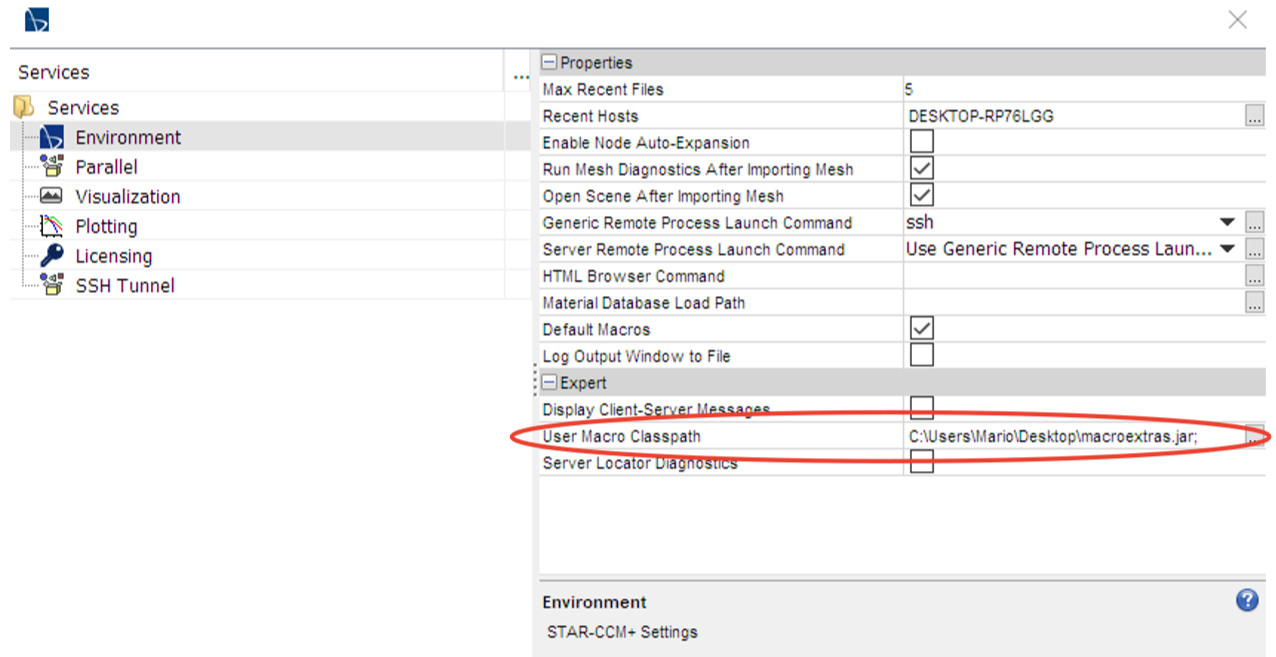
\includegraphics[scale=0.45]{Immagini/Capitolo4/starclasspath2}
\caption{\lstinline[language=Java]!MacroExtras! classpath setting inside STAR-CCM+}
\label{fig:starclasspath}
\end{figure}
%  

\section{Running STAR-CCM+ macros from inside JPAD}
\label{sec4.4}

The classes of the \lstinline[language=Java]!MacroExtras! package listed in the previous paragraph just serve as a support for the Java files in charge of the operations that actually allow to automatize the process of analysis of a certain aircraft configuration by means of a \gls{CFD} tool. The aforementioned Java files are two in number and consist of:
%
\begin{itemize}
\item a simple class providing a main method that imports some aircraft data from XML files, eventually modifies some of the components of the aircraft by means of the methods supplied by \gls{JPAD} libraries, generates a \gls{CAD} file for each of the components employing the functions offered by \lstinline[language=Java]!AircraftUtils!, writes the XML file containing all the data related to the simulation, and finally runs STAR-CCM+;
\item a STAR-CCM+ macro, which is a particular Java class that makes use of the STAR-CCM+ Macro \gls{acr:API} classes, along with the ones described in section \ref{sec4.3}, in order to perform all the operations requested before and after running an aerodynamic simulation, from importing \gls{CAD} parts into the active simulation to saving the simulation once all the calculations have been completed.
\end{itemize}
%
The following paragraphs give an overview on how these two files have been realized and on the methods and classes they make use of. The last one, in particular, just provides an example of how the main method launching the workflow can be organized, since part of its structure depends on the type of experiment/simulation that one wants to perform.

\subsection{The macro}
\label{sec4.4.1}

A STAR-CCM+ macro is a Java program that is compiled and executed within the STAR-CCM+ workspace. In order for STAR-CCM+ to actually run macros, it comes equipped with the Java \gls{acr:SDK} (the 1.7 version, so that Java 8 improvements are not available), that allows the software to compile the Java macros. The macros that one can write or record are standard Java code, meaning that it is possible to have access to all the programming constructs of the language, such as loops and conditional constructs. In addition, the STAR-CCM+ server exposes a certain number of classes, that it is possible to instantiate and manipulate in order to carry out some required sequence of tasks. Macros can be written from scratch, but that would require up-front knowledge about all the classes, attributes, and methods that the server exposes. Instead, it is more effective to use the workspace to record the actions to be performed and edit the Java file using a text editor in order to get the exact required effect.

\bigskip
\noindent
The STAR-CCM+ macro that is currently used in order to perform tests and simulations on \gls{CAD} aircraft parts produced by the use of \gls{JPAD} is called \lstinline[language=Java]!MultipleExecute!. It consists in a sequence of actions, performed in proper order, that allow to simulate fluid flow around the aforementioned aircraft components. As all the STAR-CCM+ macros, it extends the abstract class \lstinline[language=Java]!StarMacro!, and it has been included into a Java project having STAR-CCM+ \gls{JAR}s and class folders on the build path, in order for the STAR-CCM+ macros contained in this package to actually import and use STAR-CCM+ classes. For the same reason, also the path to the \lstinline[language=Java]!MacroExtras! package has been included in the build path. The \lstinline[language=Java]!MultipleExecute! macro consists of several void methods (i.e., methods that do not return anything directly), each one devoted to a specific task, and some attributes, that correspond to variables that can be used by more than one single method during the execution of the macro. As for the global variables, they are the following.
%
\begin{itemize}
\renewcommand\labelitemi{\tiny$\blacksquare$}
\renewcommand\labelitemii{\tiny$\bullet$}
\item \textbf{\lstinline[language=Java]!dataFolderPath!} - A \lstinline[language=Java]!String! variable that stands for the path to the folder in which all the files the simulation needs (the XML data file and the \gls{CAD} files in STEP format) have been stored.
\item \textbf{\lstinline[language=Java]!simFolderPath!} - A \lstinline[language=Java]!String! variable that stores the path to the directory in which the user wants to save the STAR-CCM+ simulation files. Both this and the previous variable need to be fixed by the user, in order for the macro to retrieve and save data in the proper locations.
\item \textbf{\lstinline[language=Java]!theSimulation!} - An instance of the STAR-CCM+ Macro \gls{acr:API} class \lstinline[language=Java]!Simulation!. It is the most important of the global variables of the macro, since it stores all the informations on the active simulation and it is used by all the methods across the class. It gets initialized at the very beginning of the macro, once the launching class has started running the software and played the macro.
\item \textbf{\lstinline[language=Java]!theOperatingConditions!, \lstinline[language=Java]!theGeometricData!, \lstinline[language=Java]!theSimulationParameters!} - Instances of the \lstinline[language=Java]!MacroExtras! classes \lstinline[language=Java]!OperatingConditions!, \lstinline[language=Java]!GeometricData!, and \lstinline[language=Java]!SimulationParameters! respectively. They are the variables devoted to storing all the data coming from the XML input file.
\item \textbf{\lstinline[language=Java]!thePartsMap!} - A \lstinline[language=Java]!HashMap! (an implementation of the Java \gls{Map} interface that permits null values and null keys) having keys of the \lstinline[language=Java]!ComponentEnum! type and Java \gls{List}s of strings as values. It gets initialized by means of the \lstinline[language=Java]!SimulationComponents! getter method \lstinline[language=Java]!getComponentsMap!, so it stores the file paths of each of the components that need to be imported into the active simulation. As the global variables at the previous points, it is initialized at the beginning of the macro, by the first of the methods in which \lstinline[language=Java]!MultipleExecute! macro has been split.
\item \textbf{\lstinline[language=Java]!theAircraftParts!} - A Java \gls{List} containing entities of the STAR-CCM+ \gls{acr:API} class \lstinline[language=Java]!GeometryPart!. This class, in general, manages \gls{CAD} parts once they have been imported into the simulation. So \lstinline[language=Java]!theAircraftParts! is a list containing all the imported aircraft components.
\end{itemize}
%
Listing \ref{lst:MultipleExecuteOverview} shows an overview of the macro, highlighting the attributes and the methods contained in the class. As can be seen from the listing, the macro consists of one main \lstinline[language=Java]!execute! method, which calls all the other methods present in the class in a proper sequence. Since the macro can be used also in a stand-alone way, without launching it from \gls{JPAD} but simply playing it from inside STAR-CCM+, one can think of commenting part of the tasks executed by the code, in order to have a more step-by-step approach. The following sections provide a more detailed description of some of the methods contained in the macro, especially for the ones that make greater use of Java programming constructs.
\bigskip
\begin{lstlisting}[caption={\lstinline!MultipleExecute! macro overview}, captionpos=b, tabsize=2, label={lst:MultipleExecuteOverview}]
public class MultipleExecute extends StarMacro {
	
		// Global variables
		public static final String dataFolderPath = "C:\\Users\\...";
		public static final String simFolderPath = "C:\\Users\\...";
		public static Simulation theSimulation;
		public static OperatingConditions theOperatingConditions;
		public static GeometricData theGeometricData;
		public static SimulationParameters theSimulationParameters;
		public static HashMap<ComponentEnum, List<String>> thePartsMap;
		public static List<GeometryPart> theAircraftParts;

		// Macro main method
		public void execute() {
				initializeSimulation();
				importCadParts();
				createFluidDomain();
				assignPartsToRegion();
				createReferenceValuesReports();
				createDirectionFieldFunctions();
				createMesh();
				physicsSetup();
				createAerodynamicsCoefficients();
				createBoundaryConditions();
				runSimulation();
				saveSimulation();
				killSimulation();
		}
	
		// Macro methods
		public void initializeSimulation() {
		...
		}
	
		...
	
		public void killSimulation() {
		...
		}
}	
\end{lstlisting}

\subsubsection{\texttt{initializeSimulation}}

The first of the macro methods has the fundamental task of populating global variables such as the ones related to the operating conditions, the geometric data, the simulation parameters, and the simulation components \gls{CAD} files. The method filters the files contained in the directory indicated by \lstinline[language=Java]!dataFolderPath!, distinguishing between STEP files and XML data file, and creates two distinct \lstinline[language=Java]!File! arrays, one dedicated to the \gls{CAD} components, the other one for the simulation data. The latter is used by the \lstinline[language=Java]!DataReader! class in order to initialize the global variables: \lstinline[language=Java]!theOperatingConditions!, \lstinline[language=Java]!theGeometricData!, and \lstinline[language=Java]!theSimulationParameters!. The other \lstinline[language=Java]!File! array is used by the \lstinline[language=Java]!SimulationComponents! class in order to generate a \gls{Map} to the files containing all the different \gls{CAD} components (\lstinline[language=Java]!thePartsMap!).

\subsubsection{\texttt{importCADParts}}

Once the paths to the \gls{CAD} files have been collected, it is necessary to import them into the active simulation. The STAR-CCM+ \gls{acr:API} class allowing this is \lstinline[language=Java]!PartImportManager!. Once provided with the path to the actual file and the required options (such as coincidence tolerance, merging options, and tessellation density) it imports the component, which is collected into a Java \gls{List} (\lstinline[language=Java]!theAircraftParts!) after being casted to \lstinline[language=Java]!GeometryPart!. After being imported, it is also possible to set a presentation name for the component and its surfaces, according to the name of the file from which it has been extracted. This is really helpful, since it allows in the following to get from the simulation parts list the desired part just by means of the presentation name set on it at this point. The method also automatically scales the parts according to the value set for the \lstinline[language=Java]!OperatingConditions! \lstinline[language=Java]!cadUnits! attribute. Since the \gls{OCCT} STEP writer class saves shapes in $\si{mm}$ by default, it is necessary to scale them properly.
\bigskip
\begin{lstlisting}[caption={\lstinline!importCADParts! method}, captionpos=b, tabsize=2, label={lst:importCADParts}]
public void importCadParts() {

		LabCoordinateSystem labCoordinateSystem = 
				theSimulation.getCoordinateSystemManager().getLabCoordinateSystem();
		PartImportManager partImportManager = 
				theSimulation.get(PartImportManager.class);

		int partIndex = 0;
		List<GeometryPart> aircraftParts = new ArrayList<>();
		for(Iterator<ComponentEnum> comp = 
				thePartsMap.keySet().iterator(); comp.hasNext(); ) {
			
			// Collect simulation parts into a list	
			ComponentEnum component = comp.next();		
			for(String path : thePartsMap.get(component)) {
				partImportManager.importCadPart(
						resolvePath(path), 
						"SharpEdges", 30.0, 2, true, 1.0E-5, true, false, false, false
						);
				String partName = MyStringUtils.getFilenameFromFilepath(path);
				GeometryPart aircraftPart = 
						((List<GeometryPart>) partImportManager .getParts()).get(partIndex);
				
				// Assign a proper name to the imported part and its surfaces		
				aircraftPart.setPresentationName(partName);
				((List<PartSurface>) aircraftPart.getPartSurfaces())
										.get(0)
										.setPresentationName(partName);
				
				// Scale parts whether necessary
				if(theGeometricData.getCADUnits().equals("mm")) {
					partImportManager.scaleParts(
							Collections.singletonList(aircraftPart), 
							new DoubleVector(new double[] {1000, 1000, 1000}), 
							labCoordinateSystem
							);
				}
				aircraftParts.add(aircraftPart);
				partIndex++;
			}
		}			
		
		// Initialize theAircraftParts global variable
		theAircraftParts = aircraftParts;
	}
\end{lstlisting}

\subsubsection{\texttt{createFluidDomain}}

The next step consists in creating the fluid domain in which the simulation takes place. For this purpose, a new geometry part gets created. This part is a simple block, whose dimensions are automatically set to be multiples of one of the aircraft reference length. In particular, the code set this reference length to be the greatest between the fuselage lenght and the wing span. Besides, depending on the value of the \lstinline[language=Java]!SimulationParameters! \lstinline[language=Java]!isSymmetrical! attribute, the block domain extends from the symmetry plane of the aircraft to both (positive and negative) $y$ directions or just the positive one. In addition, the front extension of the block is set to be lower than the back one, in order to let the fluid settle after having swept the aircraft. Once the block has been created, it's time to split its surface, in order to correctly assign the boundary conditions later in the code. The way the block surface gets split depends on:
%
\begin{itemize}
\item whether the simulation to be performed is symmetrical or not,
\item whether the simulation involves an inviscid flow or not,
\end{itemize}
%
with the latter condition depending on the value of the \lstinline[language=Java]!SimulationParameters! \lstinline[language=Java]!simulationType! attribute. Listing \ref{lst:createFluidDomain01} shows how the block surface gets split and how the different surfaces obtained through the process get named according to the boundary conditions to be applied onto them later. The final operation performed by the method consists in creating the actual fluid domain by means of a Boolean subtraction involving the block and the aircraft parts. The result of this operation is a new geometry part (called simply FLUID) and it is the one that it is actually used in the rest of the macro and on which operations, such as meshing and boundary conditions assignment, are performed. Its surfaces preserve the names assigned, during the previous steps, to the surfaces of the parts that have been used to generate it (i.e., the block domain and the aircraft parts), so that it is easy to retrieve them by means of the same.
\bigskip
\begin{lstlisting}[caption={Fluid domain outer surfaces creation and naming operations}, captionpos=b, tabsize=2, label={lst:createFluidDomain01}]
// Get the block surface in order to split it
PartSurface simpleBlockPartSurfaces = 
		(PartSurface) simpleBlockPart.getPartSurfaceManager()
									.getPartSurface("Block Surface");

// Split the block surface according to the simulation requirements		
if(!theSimulationParameters.isSimulationSymmetrical()) {
		
		// In case the simulation to be performed is not symmetrical
		if(theSimulationParameters.getSimulationType().equals(SimulationType.EULER)) {
		
				// In case of inviscid fluid, the back surface of the fluid block is 
				// named OUTLET, while all the remaining ones are named INLET
				simpleBlockPart.splitPartSurfaceByPatch(
					simpleBlockPartSurfaces, new IntVector(new int[] {6}), "OUTLET");
				simpleBlockPartSurfaces.setPresentationName("INLET");
		} else 
		
				// In case of viscid fluid, all the block surfaces get named FAR-FIELD
				simpleBlockPartSurfaces.setPresentationName("FAR-FIELD");
} else {	
		
		// In case the simulation to be performed is symmetrical
		if(theSimulationParameters.getSimulationType().equals(SimulationType.EULER)) {
		
				// In case of inviscid fluid, the back surface of the fluid block is named
				// OUTLET, the symmetry one is simply named SYMMETRY PLANE, and
				// the remaining ones are named INLET
				simpleBlockPart.splitPartSurfaceByPatch(
					simpleBlockPartSurfaces, new IntVector(new int[] {6}), "OUTLET");
				simpleBlockPart.splitPartSurfaceByPatch(
					simpleBlockPartSurfaces, new IntVector(new int[] {4}), "SYMMETRY PLANE");
				simpleBlockPartSurfaces.setPresentationName("INLET");
		} else {
		
				// In case of viscid fluid, the block symmetry surface is named SYMMETRY
				// PLANE, while the remaining ones are named FAR-FIELD
				simpleBlockPart.splitPartSurfaceByPatch(
					simpleBlockPartSurfaces, new IntVector(new int[] {4}), "SYMMETRY PLANE");
				simpleBlockPartSurfaces.setPresentationName("FAR-FIELD");
		}
}
\end{lstlisting}

\subsubsection{\texttt{createReferenceValuesReports} - \texttt{createDirectionFieldFunctions}}

The \lstinline[language=Java]!createReferenceValuesReports! method generates several instances of the STAR-CCM+ Macro \gls{acr:API} \lstinline[language=Java]!ExpressionReport! class, used to represent constant values that can be used throughout the macro in order to define other reports (such as those relative to aerodynamic coefficients) and to generate user defined field functions. These reports, in particular, get defined by means of the attributes of the simulation data classes \lstinline[language=Java]!OperatingConditions! and \lstinline[language=Java]!GeometricData!, with the latter being used in order to define reference lengths and surfaces. As for the user defined field functions mentioned above, they are produced by the \lstinline[language=Java]!createDirectionFieldFunctions! method and consist in directions that help defining aerodynamic coefficients. In particular, they identify the lift, drag, and side force directions by means of the angle of attack and the sideslip angle specified in the operating conditions. Both the expression reports and the direction field functions are given a specific presentation name, in order to easily retrieve them later by using it. For the sake of completeness, listing \ref{lst:DragDirectionFieldFunction} provides a sample of how direction field functions are created.
\bigskip
\begin{lstlisting}[caption={Drag direction field function}, captionpos=b, tabsize=2, label={lst:DragDirectionFieldFunction}]
// Instantiate a new field function
UserFieldFunction dragDirectionFieldFunction = 
		theSimulation.getFieldFunctionManager().createFieldFunction();
		
// Set the field function to VECTOR type
dragDirectionFieldFunction.getTypeOption()
					.setSelected(FieldFunctionTypeOption.Type.VECTOR);

// Define the direction field function by means of its components, using 
// the expression reports for the angle of attack and the sideslip angle
dragDirectionFieldFunction.setDefinition(
	"[cos(${AngleOfAttack(deg)Report}/57.3)*cos(${SideslipAngle(deg)Report}/57.3)," + 
	"sin(${SideslipAngle(deg)Report}/57.3)," + 
	"sin(${AngleOfAttack(deg)Report}/57.3)*cos(${SideslipAngle(deg)Report}/57.3)]"
	);
		
// Set an appropriate presentation name
dragDirectionFieldFunction.setFunctionName("DragDirection");
dragDirectionFieldFunction.setPresentationName("DragDirection");
\end{lstlisting} 

\subsubsection{\texttt{createMesh}}

The \lstinline[language=Java]!createMesh! method generates the discretized representation of the computational domain, which the physics solvers use to provide a numerical solution. The meshing strategy adopted by the \lstinline[language=Java]!MultipleExecute! macro is parts-based, which is a pretty common strategy for unstructured meshing: it detaches the meshing from the physics and provides a flexible and repeatable meshing pipeline. The first thing the method does is instantiating a new \lstinline[language=Java]!AutoMeshOperation! object, with \lstinline[language=Java]!AutoMeshOperation! being the STAR-CCM+ class that supervises meshing operations. The way this object is instantited depends on the type of simulation to be performed, whether it involves viscid or inviscid fluid flow. So the code contains an \emph{if} statement, whose condition is based on the \lstinline[language=Java]!SimulationParameters! \lstinline[language=Java]!simulationType! attribute. If the type of the simulation has been set to \lstinline[language=Java]!SimulationType.EULER!, the code selects the following options for the \lstinline[language=Java]!AutoMeshOperation! object.
%
\begin{itemize}
\renewcommand\labelitemi{\tiny$\blacksquare$}
\renewcommand\labelitemii{\tiny$\bullet$}
\item \textbf{Surface Remesher} - Remeshes the initial surface to provide a quality discretized mesh that is suitable for \gls{CFD}.
\item \textbf{Automatic Surface Repair} - Provides an automatic procedure for correcting a range of geometric problems that can exist in the remeshed surface once the surface remeshing process is complete.
\item \textbf{Polyhedral Mesher} - Generates a volume mesh that is composed of polyhedral-shaped cells.
\end{itemize} 
%
In addition, when the \lstinline[language=Java]!simulationType! attribute is set to \lstinline[language=Java]!SimulationType.VISCOUS!, the \textbf{Prism Layer Mesher} option gets activated. It adds prismatic cell layers next to wall boundaries, in order to capture viscous gradients at the wall. Once the \lstinline[language=Java]!AutoMeshOperation! object has been created and associated to the fluid domain part generated by the \lstinline[language=Java]!createFluidDomain! method, it is possible to set values for some of its parameters. The macro currently sets values for the following properties.
%
\begin{itemize}
\renewcommand\labelitemi{\tiny$\blacksquare$}
\renewcommand\labelitemii{\tiny$\bullet$}
\item \textbf{Base Size} - A characteristic dimension of the model that can be set before using any relative values. As for the \lstinline[language=Java]!MultipleExecute! macro, this value has been set equal to the greater between the fuselage length and the wing span.
\item \textbf{Growth Factor} - A property that defines the growth of the mesh size, whose value should be set between $1.0$ and $2.0$. Increasing its value results in larger mesh sizes in the transition from boundary size to the size away from the boundary. The macro currently sets its value to $1.3$.
\end{itemize}
%
In case of viscid fluid flow, the macro also automatically sets values regarding the Prism Layer Mesher. In particular, it sets the number of prism layers (currently fixed to $10$) and the absolute prism layer thickness, to calculate the value of which the macro uses the formula for turbulent boundary layers over a flat plate:
\[
\delta \approx 0.37x/{\text{Re}}_{x}^{1/5}
\]
with the Reynolds number based on the reference length expression report created by the \lstinline[language=Java]!createReferenceValuesReports! method (and equal to the wing mean aerodynamic chord). The last operations performed by the method consist in generating custom mesh controls for the aircraft part surfaces  the fluid domain is made up of. In general, surface custom mesh controls override any default controls for the volume mesher, allowing to refine or coarsen the mesh for part surfaces. The custom controls the macro makes use of are the following.
%
\begin{itemize}
\renewcommand\labelitemi{\tiny$\blacksquare$}
\renewcommand\labelitemii{\tiny$\bullet$}
\item \textbf{Target Surface Size} - Defines the edge length that the mesher aims for in absence of any mesh refinement. Decreasing the target surface size generates more refined and detailed surface mesh.
\item \textbf{Minimum Surface Size} - Specifies the lower limit of edge lengths on the surface mesh. Decreasing the minimum surface size allows more refinement in regions where the mesher is trying to capture complex features.
\end{itemize}
% 
The \lstinline[language=Java]!MultipleExecute! macro specifies the controls listed above for each aircraft surface and as relative to the aforementioned base size. Besides, the code automatically detects the type of the surface the controls are being set for, and uses different values depending on which part surfaces belong to. For example, the values used for the fuselage are five times the ones used for the lifting surfaces in general (target surface size equal to $0.1$ of the base size, minimum surface size equal to $0.01$ of the base size), since the latter typically require much more mesh refinement.
%
\bigskip
\begin{figure}[H]
\centering
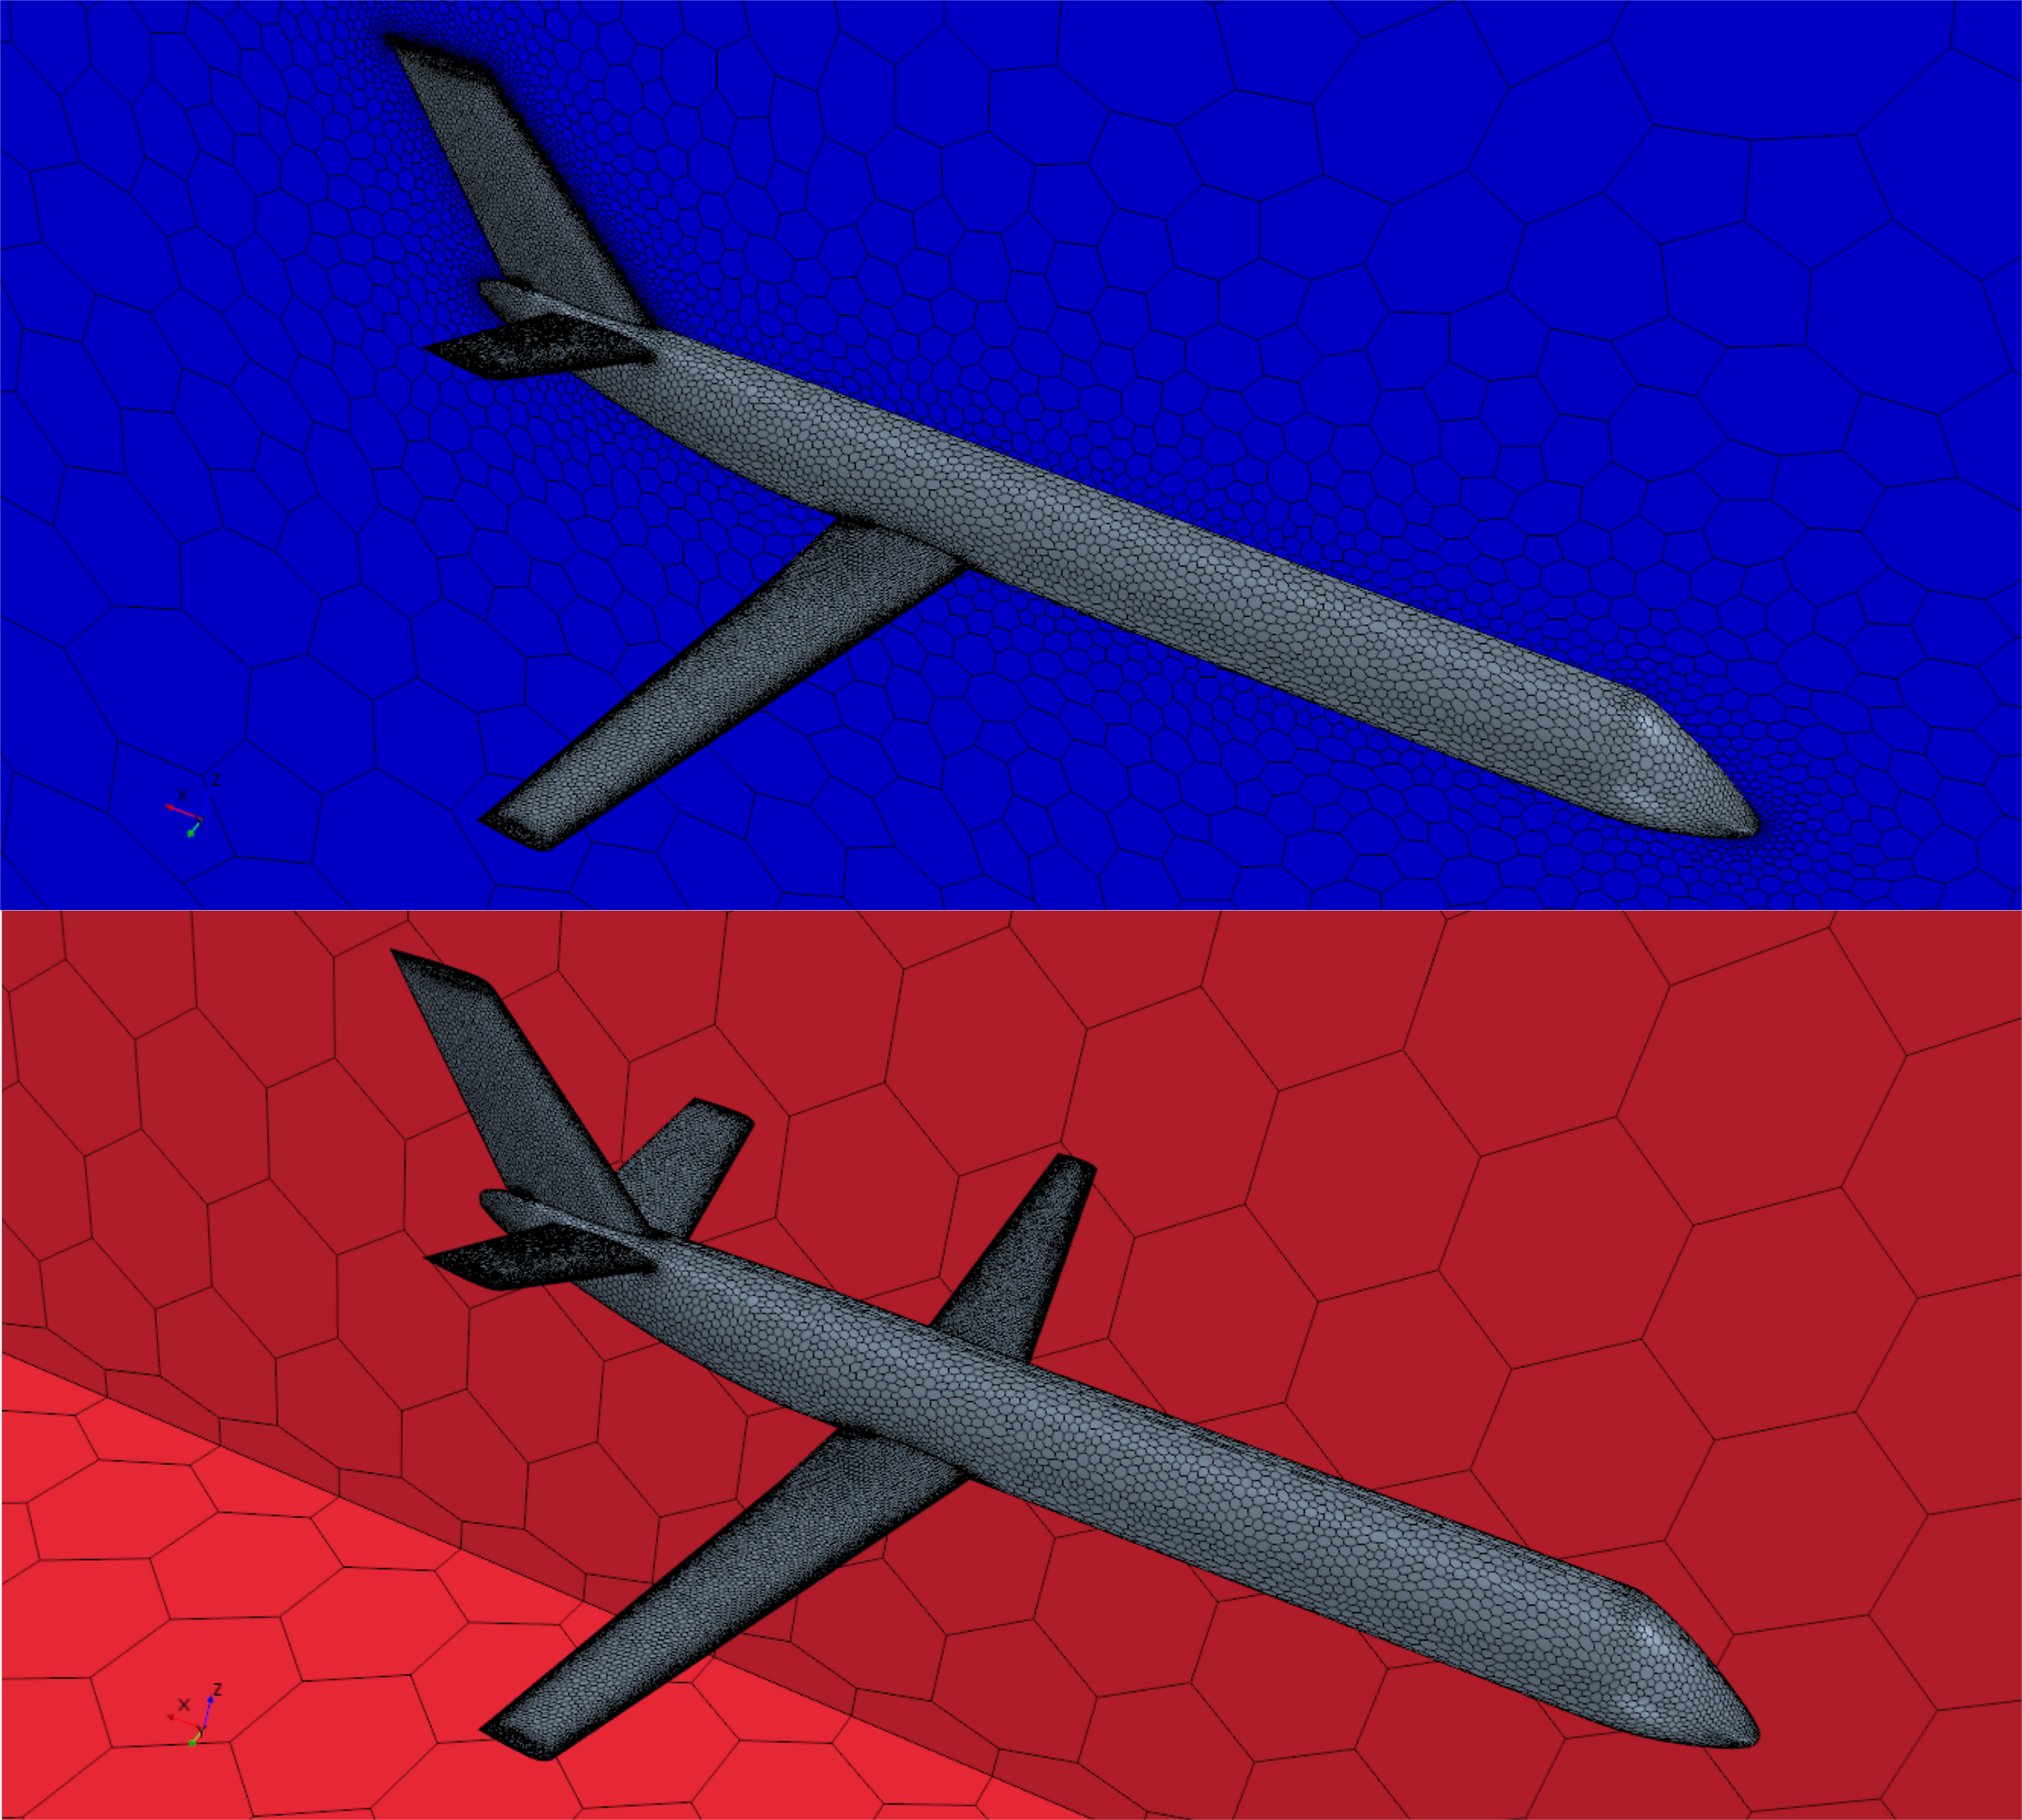
\includegraphics[scale=0.60]{Immagini/Capitolo4/symmetry}
\caption{Automated meshes for symmetrical/non-symmetrical simulations}
\label{fig:SymmMesh}
\end{figure} 
%
\begin{figure}[H]
\centering
\includegraphics[scale=0.60]{Immagini/Capitolo4/airfoil}
\caption{Automated meshes for non-viscous/viscous fluid flows}
\label{fig:AirfoilMesh}
\end{figure} 
%

\subsubsection{\texttt{physicsSetup}}

Once the meshing operations have been defined (altough the actual mesh still needs to be generated), the macro arranges for the set up of the physics models. These define the primary variables of the simulation and what mathematical formulation is used to generate the solution. An appropriate combination of models is necessary for the complete definition of a physics continuum. After generating a new \lstinline[language=Java]!PhysicsContinuum! object, with \lstinline[language=Java]!PhysicsContinuum! being the class that manages physics models definition, the method enables several physics models, common to both viscid and inviscid flow simulations. Then an \emph{if} statement allows to select different models depending on the value of the \lstinline[language=Java]!SimulationParameters! \lstinline[language=Java]!simulationType! attribute. In case the attribute is equal to \lstinline[language=Java]!SimulationType.EULER!, the Inviscid Model is enabled. If not, several models relative to turbulence and its treatment get implemented. Listing \ref{lst:PhysicsSetup} reports the whole method, along with the list of physics models enabled by the macro.
\bigskip
\begin{lstlisting}[caption={\lstinline!physicsSetup! method}, captionpos=b, tabsize=2, label={lst:PhysicsSetup}]
public void physicsSetup() {

		// Generate a new instance of PhysicsContinuum
		PhysicsContinuum physicsContinuum = 
				theSimulation.getContinuumManager().createContinuum(PhysicsContinuum.class);
		physicsContinuum.setPresentationName("Physics");
		
		// Enable some basic physics models
		physicsContinuum.enable(ThreeDimensionalModel.class);
		physicsContinuum.enable(SteadyModel.class);
		physicsContinuum.enable(SingleComponentGasModel.class);
		physicsContinuum.enable(CoupledFlowModel.class);
		physicsContinuum.enable(IdealGasModel.class);
		physicsContinuum.enable(CoupledEnergyModel.class);
		
		// Enable more specific physics models
		if(theSimulationParameters.getSimulationType().equals(SimulationType.VISCOUS)) {
			physicsContinuum.enable(TurbulentModel.class);
			physicsContinuum.enable(RansTurbulenceModel.class);
			physicsContinuum.enable(SpalartAllmarasTurbulence.class);
			physicsContinuum.enable(SaTurbModel.class);
			physicsContinuum.enable(SaAllYplusWallTreatment.class);
		} else {
			physicsContinuum.enable(InviscidModel.class);
		}	
		
		// Set a value for the reference pressure
		physicsContinuum.getReferenceValues()
					.get(ReferencePressure.class)
					.setValue(theOperatingConditions.getPressure());
}
\end{lstlisting}  

\subsubsection{\texttt{createAerodynamicsCoefficients}}

The expression reports and the direction field functions created by the methods described above are mostly used in order to define aerodynamic coefficients. \lstinline[language=Java]!ForceCoefficientReport! and \lstinline[language=Java]!MomentCoefficientReport! are the STAR-CCM+ classes that help creating this kind of entities. These coefficients, in order to be properly defined, need to be associated to the surfaces on which they are calculated. All the coefficients defined at this point are calculated on the whole aircraft. Listing \ref{lst:createAerodynamicsCoefficients} shows how the lift coefficient and the pitch moment coefficient reports are defined. It has to be noted that the reference surface area gets automatically adjusted in case the simulation to be performed is symmetrical. In addition to the reports for the aerodynamic coefficients, the method also provides the definitions for the pressure coefficient (by means of the \lstinline[language=Java]!PressureCoefficientFunction! class) and, in case \lstinline[language=Java]!simulationType! is set to \lstinline[language=Java]!VISCOUS!, the skin friction coefficient (by means of the \lstinline[language=Java]!SkinFrictionCoefficientFunction! class).
\bigskip
\begin{lstlisting}[caption={Force and moment coefficients creation}, captionpos=b, tabsize=2, label={lst:createAerodynamicsCoefficients}]
// Generate a new force coefficient instance
ForceCoefficientReport liftCoefficientReport 
		= theSimulation.getReportManager().createReport(ForceCoefficientReport.class);
		
// Set a direction by means of the field function created before	
liftCoefficientReport.getDirection().setDefinition("$${LiftDirection}");

// Set reference quantities by means of the expression reports created above
liftCoefficientReport.getReferenceDensity().setDefinition(
		"${DensityReport}");
liftCoefficientReport.getReferenceVelocity().setDefinition(
		"${ReferenceVelocityReport}");
liftCoefficientReport.getReferenceArea().setDefinition(
		"${ReferenceAreaReport}/" + Integer.toString(symmetryFactor));

// Set the surface
liftCoefficientReport.getParts().setObjects(aircraftBoundaries);

// Set the presentation name
liftCoefficientReport.setPresentationName("CL");

// Generate a new moment coefficient instance
MomentCoefficientReport pitchMomentCoefficientReport = 
		theSimulation.getReportManager().createReport(MomentCoefficientReport.class);

// Set a direction by using components		
pitchMomentCoefficientReport.getDirection().setComponents(0.0, 1.0, 0.0);

// Set reference quantities by means of the expression reports created above
pitchMomentCoefficientReport.getReferenceDensity().setDefinition(
		"${DensityReport}");
pitchMomentCoefficientReport.getReferenceVelocity().setDefinition(
		"${ReferenceVelocityReport}");
pitchMomentCoefficientReport.getReferenceRadius().setDefinition(
		"${ReferenceLengthReport}");
pitchMomentCoefficientReport.getReferenceArea().setDefinition(
		"${ReferenceAreaReport}/" + Integer.toString(symmetryFactor));

// Set the pole
pitchMomentCoefficientReport.getOrigin().setDefinition(
		"[${ReferenceMomentPoleReport}, 0.0, 0.0]");

// Set the surface
pitchMomentCoefficientReport.getParts().setObjects(aircraftBoundaries);

// Set the presentation name
pitchMomentCoefficientReport.setPresentationName("CM");
\end{lstlisting}

\subsubsection{\texttt{createBoundaryConditions}}

Before finally being able to run the simulation, boundary conditions must be applied. Since the fluid domain surface has already been split by one of the previous methods, at this point it's just necessary to impose proper conditions, based on the name given to the surfaces by the same method. For this purpose, \lstinline[language=Java]!createBoundaryConditions! performs a first check on the symmetry of the problem: if so, a symmetry boundary condition is applied on the fluid domain surface previously named SYMMETRY PLANE (listing \ref{lst:createFluidDomain01}). Then, an \emph{if} statement, whose condition depends on the \lstinline[language=Java]!simulationType! attribute, helps the code deciding which boundary conditions should be applied on the remaining surfaces. If the simulation to be performed involves inviscid fluid, velocity inlet and pressure outlet boundary conditions are applied on the surfaces previously named INLET and OUTLET respectively. Otherwise, a free-stream condition is applied on the FAR-FIELD surfaces of the fluid domain. As for the aircraft surfaces, a wall boundary condition is applied automatically, so there's no need to modify anything. In order to set values for the quantities that it is necessary to define for each of the boundary conditions mentioned above, expression reports and direction field functions are used. Listing \ref{lst:CreateBoundaryConditions} shows the entire method, along with the quantities defined for the boundary conditions.
\bigskip
\begin{lstlisting}[caption={\lstinline!createBoundaryConditions! method}, captionpos=b, tabsize=2, label={lst:CreateBoundaryConditions}]
public void createBoundaryConditions() {
	
	// Instantiate a new BoundaryManager object
	BoundaryManager boundaryManager 
			= theSimulation.getRegionManager().getRegion("Region").getBoundaryManager();

	// Checking on symmetry		
	if(theSimulationParameters.isSimulationSymmetrical()) {
	
		// Get the symmetry surface by means of its 
		// presentation name and set its boundary type
		boundaryManager.getBoundary("FLUID.Block.SYMMETRY PLANE")
			.setBoundaryType(
				(SymmetryBoundary) theSimulation.get(ConditionTypeManager.class)
									.get(SymmetryBoundary.class));
	}
		
	// Simulation type check	
	if(theSimulationParameters.getSimulationType().equals(SimulationType.EULER)) {
	
		// In case of inviscid fluid flow		
		Boundary inflow = boundaryManager.getBoundary("FLUID.Block.INLET");
		Boundary outflow = boundaryManager.getBoundary("FLUID.Block.OUTLET");

		inflow.setBoundaryType(
			(InletBoundary) theSimulation.get(ConditionTypeManager.class)
									.get(InletBoundary.class));		
		outflow.setBoundaryType(
			(PressureBoundary) theSimulation.get(ConditionTypeManager.class)
									.get(PressureBoundary.class));
									
		// Set definitions for velocity inlet BC quantities
		inflow.getConditions().get(FlowDirectionOption.class)
						.setSelected(FlowDirectionOption.Type.COMPONENTS);
		inflow.getValues().get(FlowDirectionProfile.class)
						.getMethod(ConstantVectorProfileMethod.class)
						.getQuantity().setDefinition("$${DragDirection}");
		inflow.getValues().get(StaticTemperatureProfile.class)
						.getMethod(ConstantScalarProfileMethod.class)
						.getQuantity().setDefinition("${TemperatureReport}");
		inflow.getValues().get(VelocityMagnitudeProfile.class)
						.getMethod(ConstantScalarProfileMethod.class)
						.getQuantity().setDefinition("${ReferenceVelocityReport}");
		
		// Set definitions for pressure outlet BC quantities
		outflow.getValues().get(StaticTemperatureProfile.class)
						.getMethod(ConstantScalarProfileMethod.class)
						.getQuantity().setDefinition("${TemperatureReport}");
	} else {
	
		// In case of viscous fluid flow
		Boundary freeStream = boundaryManager.getBoundary("FLUID.Block.FAR-FIELD");

		freeStream.setBoundaryType(
			(FreeStreamBoundary) theSimulation.get(ConditionTypeManager.class)
									.get(FreeStreamBoundary.class));
		
		// Set definitions for free-stream BC quantities
		freeStream.getValues().get(FlowDirectionProfile.class)
						.getMethod(ConstantVectorProfileMethod.class)
						.getQuantity().setDefinition("$${DragDirection}");
		freeStream.getValues().get(MachNumberProfile.class)
						.getMethod(ConstantScalarProfileMethod.class)
						.getQuantity().setDefinition("${MachNumberReport}");
		freeStream.getValues().get(StaticTemperatureProfile.class)
						.getMethod(ConstantScalarProfileMethod.class)
						.getQuantity().setDefinition("${TemperatureReport}");
	}
}
\end{lstlisting}

\subsubsection{\texttt{runSimulation} - \texttt{saveSimulation} - \texttt{killSimulation}}

The three last methods allow, respectively, to generate the mesh and run the simulation (whether the \lstinline[language=Java]!executeMesh! attribute has been set to \lstinline[language=Java]!TRUE!), to save the simulation with a proper name, and to kill the simulation. The last step is fundamental when playing the macro in batch mode, because it allows to properly close the active simulation, in order to start a new one or simply end the process.

\subsection{The launching class}
\label{sec4.4.2}

The last piece of the puzzle consists of the Java class which, equipped with a main method and a series of attributes used as global variables, allows to launch a simulation (or a cycle of simulations) from within \gls{JPAD}. It is necessary to point out that the class described below provides only an example of how the main method should be structured for simulation purposes. In particular, the class described in the following corresponds to the one used for testing out the macro described in the previous paragraph and the system of classes provided by \lstinline[language=Java]!MacroExtras!. 

\bigskip
\noindent
First thing, the launching class requires some attributes to be set. These attributes, corresponding to instances of the Java \lstinline[language=Java]!String! class, are the following.
%
\begin{itemize}
\renewcommand\labelitemi{\tiny$\blacksquare$}
\item \textbf{\lstinline[language=Java]!workingFolderPath!} - Defines the path to the folder in which \gls{CAD} files are stored, along with the XML file containing all the information about the simulation to be run.
\item \textbf{\lstinline[language=Java]!jpadCADFolder!} - Defines the path to the folder in which \gls{JPAD} \gls{CAD} files are generated and initially stored.
\item \textbf{\lstinline[language=Java]!macroPath!} - Contains the path of the folder in which the custom macros are stored (\lstinline[language=Java]!MultipleExecute! is one of them).
\item \textbf{\lstinline[language=Java]!macroName!} - A string standing for the name of the macro to be run.
\item \textbf{\lstinline[language=Java]!starExePath!} - Defines the path to the STAR-CCM+ .exe file.
\item \textbf{\lstinline[language=Java]!starOptions!} - A Java \lstinline[language=Java]!String! containing a set of option for STAR-CCM+ execution, like the path to the software license and the number of processors that must be used during the simulation.
\end{itemize}
%
As for the main method of the class, the first operation performed consists in loading an aircraft from XML data file. For this purpose, the \lstinline[language=Java]!AircraftUtils.importAircraft! method is used, once the launching class run configuration has been provided with an appropiate set of arguments (see section \ref{sec3.6}). After the aircraft has been correctly imported, what the code makes is building a \gls{Map}, called \lstinline[language=Java]!aeroMap!, similar to the one produced by the \lstinline[language=Java]!SimulationComponents! class: it contains \lstinline[language=Java]!MacroExtras! \lstinline[language=Java]!ComponentEnum! constants as keys to Java \gls{List}s of generic objects, which can be instances of \gls{JPAD} \lstinline[language=Java]!Fuselage! and \lstinline[language=Java]!LiftingSurface! classes. The actual \gls{Map} implementation used in the code is the \lstinline[language=Java]!ConcurrentHashMap!, which allows concurrent modification of the \gls{Map} and allows it to be modified during iteration. Listing \ref{lst:AeroMap} shows how this \gls{Map} is created. It is important to note that each key is associated to a list and not to just a single entity, in accordance with the way in which the \lstinline[language=Java]!MacroExtras! classes and the \lstinline[language=Java]!MultipleExecute! macro have been arranged. This means that, for example, one can think of chosing one of the aircraft components present in \lstinline[language=Java]!aeroMap!, generate a copy of the original one and modify it by means of the methods offered by the \gls{JPAD} library, and finally add it to \lstinline[language=Java]!aeroMap!, as listing \ref{lst:AddCustomComponents} shows.
%
\bigskip
\begin{lstlisting}[caption={Aircraft Map creation}, captionpos=b, tabsize=2, label={lst:AeroMap}]
// Import aircraft data from file
Aircraft aircraft = AircraftUtils.importAircraft(args);	

// Generate the Map and populate it with keys 
// and empty Lists of generic Java Object entities	
ConcurrentHashMap<ComponentEnum, List<Object>> aeroMap 
		= new ConcurrentHashMap<ComponentEnum, List<Object>>();
aeroMap.put(ComponentEnum.FUSELAGE, new ArrayList<Object>());
aeroMap.put(ComponentEnum.WING, new ArrayList<Object>());
aeroMap.put(ComponentEnum.CANARD, new ArrayList<Object>());
aeroMap.put(ComponentEnum.HORIZONTAL, new ArrayList<Object>());
aeroMap.put(ComponentEnum.VERTICAL, new ArrayList<Object>());

// Iterate through the Map, adding Fuselage and LiftingSurface  
// objects to the initially empty Lists whether necessary			
for(Iterator<ComponentEnum> comp = aeroMap.keySet().iterator(); comp.hasNext(); ) {
			
	ComponentEnum component = comp.next();
	switch(component) {
	
	// Add fuselages to the Map		
	case FUSELAGE:
		if(!(aircraft.getFuselage() == null))
			aeroMap.get(ComponentEnum.FUSELAGE).add(aircraft.getFuselage());
		else {
			System.out.println("There's no FUSELAGE component for the selected aircraft");
			aeroMap.remove(component);
		}
				
		break;
	
	// Add wings to the Map			
	case WING:
		if(!(aircraft.getWing() == null))
			aeroMap.get(ComponentEnum.WING).add(aircraft.getWing());
		else {
			System.out.println("There's no WING component for the selected aircraft");
			aeroMap.remove(component);
		}
				
		break;
				
	...
	}
}
\end{lstlisting}
%
\bigskip
\begin{lstlisting}[caption={Adding custom components to the original Map}, captionpos=b, tabsize=2, label={lst:AddCustomComponents}]
// Chose to add a custom canard, if the original aircraft has one
ComponentEnum customComponentEnum = ComponentEnum.CANARD;
if(aeroMap.containsKey(customComponentEnum)) {
		
	// Return in case it has been decided to add a custom fuselage	
	if(customComponentEnum.equals(ComponentEnum.FUSELAGE)) return;
	
	// Initialize the original component and the custom component		
	LiftingSurface originalComponent = (LiftingSurface) aeroMap
											.get(customComponentEnum).get(0);
	LiftingSurface customComponent = null;
	
	// Reimport the component to be modified		
	switch(customComponentEnum.name()) {
			
	case "WING": 
		customComponent = AircraftUtils.importAircraft(args).getWing();
		break;
						
	...

	}
	
	// Modify the chosen component by means of JPAD methods and criteria				
	customComponent.adjustDimensions(
			originalComponent
					.getAspectRatio()*1.2,
			originalComponent.getEquivalentWing().getPanels().get(0)
					.getChordRoot().doubleValue(SI.METER)*1.1,
			originalComponent.getEquivalentWing().getPanels().get(0)
					.getChordTip().doubleValue(SI.METER)*0.9, 
			originalComponent.getEquivalentWing().getPanels().get(0)
					.getSweepLeadingEdge(),
			originalComponent.getEquivalentWing().getPanels().get(0)
					.getDihedral(), 
			originalComponent.getEquivalentWing().getPanels().get(0)
					.getTwistGeometricAtTip(), 
			WingAdjustCriteriaEnum.AR_ROOTCHORD_TIPCHORD
			);
	
	// Set the airfoil list for the custom component		
	customComponent.setAirfoilList(originalComponent.getAirfoilList());	
	
	// Set the coordinates for the construction axes origin of the custom component
	customComponent.setXApexConstructionAxes(
			originalComponent.getXApexConstructionAxes()
			.plus(Amount.valueOf(3, SI.METER)));
	customComponent.setYApexConstructionAxes(
			originalComponent.getYApexConstructionAxes());
	customComponent.setZApexConstructionAxes(
			originalComponent.getZApexConstructionAxes()
			.plus(Amount.valueOf(0.1, SI.METER)));
	
	// Finally add the custom component to the Map
	aeroMap.get(customComponentEnum).add(customComponent);
}
\end{lstlisting}
%

\bigskip
\noindent
Once all has been set on the aircraft components side, it's necessary to fix the simulation data by means of the classes provided by \lstinline[language=Java]!MacroExtras!. For this purpose, three new instances of the classes listed in section \ref{sec4.3.2} are created. As for the geometric data, the getter methods provided by the \lstinline[language=Java]!Fuselage! and \lstinline[language=Java]!LiftingSurface! classes are used. Besides, a check is made on the components contained in the aircraft \gls{Map}: if no fuselage is present, the fuselage length attribute of the \lstinline[language=Java]!GeometricData! class is automatically set to zero (so that the macro showed in the previous paragraph always choses the wing span as the reference length), while if no wing is present among the keys list of \lstinline[language=Java]!aeroMap! the code flow is stopped and the main method of the STAR-CCM+ macro launching class returns nothing. As for the operating conditions, instead, the launching class makes use of two of \gls{JPAD} utility classes, \lstinline[language=Java]!AtmosphCalc! and \lstinline[language=Java]!StdAtmos1976!, which provide methods for calculating the atmospheric properties of the \gls{acr:ICAO} 1976 Standard Atmosphere to an arbitrary altitude. Once everything is ready, the builders of the simulation data classes provide the methods to be used in order to generate the objects to be passed to the \lstinline[language=Java]!DataWriter! class (listing \ref{lst:OperCond01} and \ref{lst:DatWrit01}).
%
\bigskip
\begin{lstlisting}[caption={Instantiate a new \lstinline!OperatingConditions! object}, captionpos=b, tabsize=2, label={lst:OperCond01}]
// Define the operating conditions
double angleOfAttack = 2.0;
double sideslipAngle = 0.0;
double machNumber = 0.64;
double altitude = 30000; 
double altitudeM = Amount.valueOf(altitude, NonSI.FOOT)
						.doubleValue(SI.METER);
		
StdAtmos1976 atmosphere = AtmosphereCalc.getAtmosphere(altitudeM);
double pressure = atmosphere.getPressure();
double density = atmosphere.getDensity()*1000;
double temperature = atmosphere.getTemperature();
double speedOfSound = atmosphere.getSpeedOfSound();
double dynamicViscosity = AtmosphereCalc.getDynamicViscosity(altitudeM);
double velocity = speedOfSound*machNumber;
double reynoldsNumber = density*velocity*wingMAC/dynamicViscosity;

// Generate the operating conditions object
OperatingConditions operatingConditions = 
		new OperatingConditions.OperatingConditionsBuilder()
				.setAngleOfAttack(angleOfAttack)
				.setSideslipAngle(sideslipAngle)
				...
				.setVelocity(velocity)
				.build();
\end{lstlisting}
%
\bigskip
\begin{lstlisting}[caption={Instantiate a new \lstinline!DataWriter! object}, captionpos=b, tabsize=2, label={lst:DatWrit01}]
// Create the data file writer
DataWriter writer = new DataWriter(
		operatingConditions, 
		geometricData, 
		simulationParameters			
		);
\end{lstlisting}
%

\bigskip
\noindent
The XML data file is not the only file that the launching class needs to generate. By means of the utilities listed in Chapter \ref{chap3}, it also generates the \gls{CAD} files, in STEP format, containing the solid counterparts of the components listed in \lstinline[language=Java]!aeroMap!. What the launching class does, in particular, is to iterate through the keys of the aircraft components \gls{Map}, chosing for each key the right method and the proper options to be set for it, depending on the type of the component to be converted to \gls{CAD} file. Listing \ref{lst:AircraftCADFiles} shows an excerpt of the original code in which the operations just described are performed. It has to be noted that also the name each file is given is chosen precisely, because from it depends the right functioning of the macro, as described in the previous paragraph.
%
\bigskip
\begin{lstlisting}[caption={Aircraft components CAD files generation}, captionpos=b, tabsize=2, label={lst:AircraftCADFiles}]
// Create aircraft CAD files
List<String> cadNames = new ArrayList<>();
		
// Iterate through aircraft components Map keys
for(Iterator<ComponentEnum> comp = aeroMap.keySet().iterator(); comp.hasNext(); ) {
	ComponentEnum component = comp.next();
			
	switch(component.name()) {
	
	// Transfer fuselage shapes to CAD file		
	case "FUSELAGE":
		int nFus = aeroMap.get(component).size();				 
		for(int i = 0; i < nFus; i++) {
			String cadName = (nFus > 1) ? ("FUSELAGE_" + (i + 1)) : "FUSELAGE";
			cadNames.add(cadName);
			AircraftUtils.getAircraftSolidFile(
				AircraftUtils.getFuselageCAD(
					(Fuselage) aeroMap.get(component).get(i), 
					7, 7, true, true, false), 
				cadName, 
				FileExtension.STEP);
		}
		break;
	
	// Transfer wing shapes to CAD file			
	case "WING":
		int nWng = aeroMap.get(component).size();				 
		for(int i = 0; i < nWng; i++) {
			String cadName = (nWng > 1) ? ("WING_" + (i + 1)) : "WING";
			cadNames.add(cadName);
			AircraftUtils.getAircraftSolidFile(
				AircraftUtils.getLiftingSurfaceCAD(
					(LiftingSurface) aeroMap.get(component).get(i), 
					ComponentEnum.WING, 1e-3, false, true, false), 
				cadName, 
				FileExtension.STEP);
		}
		break;				
	...
}
\end{lstlisting}
%

\bigskip
\noindent
At this point, all the necessary preparations for the launch of the macro are almost over. What remains to be done is to make copies of the \gls{CAD} files generated at the previous step and move them to the folder in which all the simulation files are stored (\lstinline[language=Java]!workingFolderPath!). Besides, it is necessary to actually write to XML file format the simulation data. This operation can be performed by using the \lstinline[language=Java]!write! method supplied by the \lstinline[language=Java]!DataWriter! class. Finally, the macro can be played by running the STAR-CCM+ application in batch mode. The Java classes allowing this are \lstinline[language=Java]!Runtime! and \lstinline[language=Java]!Process!. By means of the former the application (i.e., the launching class) is allowed to interface with the environment in which it is running. The \lstinline[language=Java]!getRuntime! method of this class simply returns the runtime object associated with the current Java application, which can be used in order to execute commands provided to the \lstinline[language=Java]!Runtime! class \lstinline[language=Java]!exec! method in the form of strings. The usage of this method produces an instance of the \lstinline[language=Java]!Process! class, which allows to perform input from the process, perform output to the process, wait for the process to complete, check the exit status of the process, and destroy (kill) the process. Listing \ref{lst:RunningSTAR} shows precisely how the procedure described above has been coded.
%
\bigskip
\begin{lstlisting}[caption={Launching class final steps}, captionpos=b, tabsize=2, label={lst:RunningSTAR}]
// Copy the CAD files and move them to the working folder
cadNames.forEach(s -> {
	try { 
		Files.copy(		
			Paths.get(jpadCADFolder + "\\" + s + ".step"), 
			Paths.get(workingFolderPath + "\\" + s + ".step"), 
			StandardCopyOption.REPLACE_EXISTING
			);
	} 
	catch (IOException e) {
		e.printStackTrace();
	}
});

// Write simulation data to XML file format		
writer.write(workingFolderPath + "\\Data.xml");
		
// Run STAR-CCM+ application in batch mode 
// and play MultipleExecute Java macro
try {
	// Get the runtime object
	Runtime runtime = Runtime.getRuntime();
		
	// Execute commands	
	Process runTheMacro = runtime.exec(
		"cmd /c cd\\ && cd " + macroPath + " && dir && " + // change directory
		"\"" + starExePath + "\" " +  // run the application
		starOptions + " " +  // set license and settings
		"-new -batch " + macroName // start new simulation in batch mode
		); 
	
	// Get the input from the running process and print it to console		         
	BufferedReader input = 
		new BufferedReader(new InputStreamReader(runTheMacro.getInputStream()));
            
        String line = null;		
	while((line = input.readLine()) != null) System.out.println(line);
		
	// Exit the process once all the operations prescribed  
	// by the previous step have been completed	
	int exitVal = runTheMacro.waitFor();
        System.out.println("Exited with error code " + exitVal);
}
		
catch(Exception e) {
	System.out.println(e.toString());
	e.printStackTrace();
}
\end{lstlisting}
%

\bigskip
\noindent
The steps listed above show how to launch a single simulation starting from a dedicated class contained in \gls{JPAD}, making use of the \lstinline[language=Java]!MacroExtras! classes and a STAR-CCM+ macro specifically written for the purpose. At this point it is immediate to think that such an operation can be launched several times consecutively, employing the loop statements offered by the Java language, for the purpose of, for example, studying the contribution to the aerodynamics of the aircraft offered by lifting surfaces with different characteristics or simply positioned in an alternative manner (and it has been seen right above, listing \ref{lst:AddCustomComponents}, how the \lstinline[language=Java]!Fuselage! and \lstinline[language=Java]!LiftingSurface! classes through their methods easily allow to act on aircraft components parameters). Figure \ref{fig:STARJPADWorkflow} summarizes these concepts, offering an overview of how a workflow involving the \gls{JPAD} library and the STAR-CCM+ analysis tools could be arranged.
%
\begin{figure}[H]
\centering
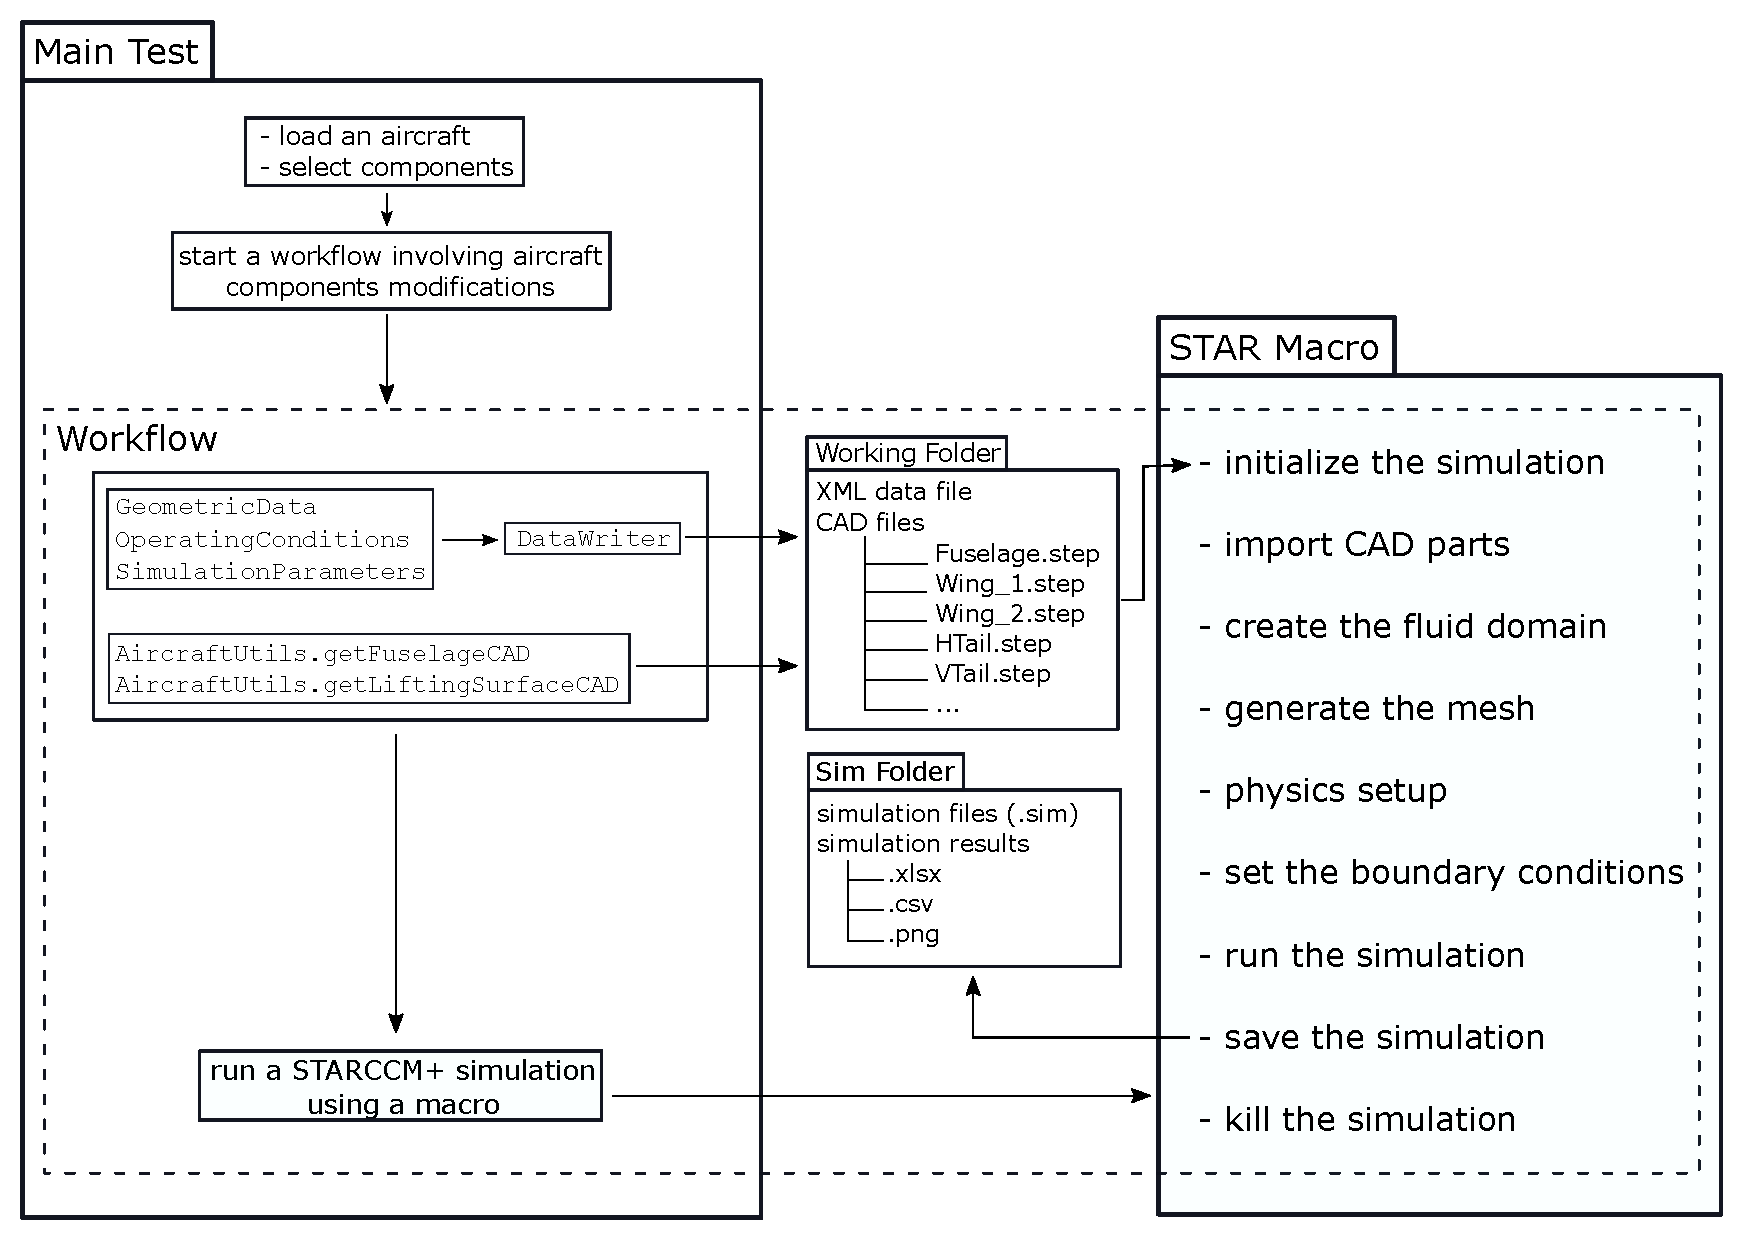
\includegraphics[scale=0.50]{Immagini/Capitolo4/starworkflow}
\caption{JPAD - STAR-CCM+ workflow overview}
\label{fig:STARJPADWorkflow}
\end{figure}
%  

\subsection{Interoperability example}
\label{sec4.4.3}

The following tables and pictures show an example of usage of the framework described in this chapter. The simulations (involving an inviscid fluid flow) have been performed on an innovative configuration developed by the DAF research group as part of the IRON Project. The code explained in the previous chapter has been used in order to modify the aircraft configuration. More in general, \gls{CFD} analyses performed on \gls{CAD} components generated by means of \lstinline[language=Java]!JPADCAD! and \lstinline[language=Java]!AircraftUtils! have returned plausible results, and in accordance with the ones obtained for more refined \gls{CAD} models. However, still more tests are needed in this sense, especially for simulations involving viscous flow.
%
\bigskip
\begin{table}[H]
\centering
\begin{tabular}{lr}
\toprule
\multicolumn{2}{c}{\textbf{Operating Conditions}} \\
\midrule
$\alpha$ & $\SI{2}{\degree}$ \\
$\beta$ & $\SI{0}{\degree}$ \\
$\text{M}$ & $0.64$\\
$h$ & $\SI{30000}{\foot}$ \\
$V$ & $\SI{194.07}{\meter\per\second}$ \\
\bottomrule
\end{tabular}
\caption{Operating conditions for both the tests}
\label{tab:Operating_Conditions}
\end{table}
%
\begingroup
\begin{longtable}[h]{lr}
\textbf{} & \textbf{Geometric data} \\
\toprule
\endfirsthead
%
\multicolumn{2}{l}%
  {\relsize{-1}({\itshape continued from previous page})}\\
 \textbf{} & \textbf{Geometric data} \\
\toprule
\endhead
%
\midrule \multicolumn{2}{r}{{\relsize{-1}\itshape continued on next page}}
\endfoot
%
\bottomrule
\caption{Aircraft data}
\endlastfoot
%
\textbf{Fuselage} & \textbf{ } \\
\midrule
Total Length & $\SI{38.04}{\meter}$ \\
Cylinder Diameter & $\SI{3.510}{\meter}$ \\
\midrule
\textbf{Wing} & \textbf{ } \\
\midrule
Planform Surface & $\SI{98.6}{\square\meter}$ \\
\AR & 11.96 \\
Span & $\SI{34.34}{\meter}$ \\
Mean Aerodynamic Chord & $\SI{3.05}{\meter}$ \\
Twist at Root & $\SI{0.0}{\degree}$ \\
Twist at Tip & $\SI{-2.0}{\degree}$ \\
\midrule
\textbf{Horizontal Tail} & \textbf{ } \\
\midrule
Planform Surface & $\SI{39.91}{\square\meter}$ \\
\AR & 4.261 \\
Span & $\SI{13.04}{\meter}$ \\
\midrule
\textbf{Vertical Tail} & \textbf{ } \\
\midrule
Planform Surface & $\SI{24.45}{\square\meter}$ \\
\AR &  1.366 \\
Span & $\SI{5.78}{\meter}$ \\
\midrule
\textbf{Canard} & \textbf{ } \\
\midrule
Planform Surface & $\SI{10.974}{\square\meter}$ \\
\AR &  5.125 \\
Span & $\SI{7.5}{\meter}$ \\
\end{longtable}
\endgroup
%
\bigskip
\begin{table}[H]
\centering
\begin{tabular}{lrrr}
\toprule
\textbf{Part} & \textbf{$C_{L}$} & \textbf{$C_{D}$} & \textbf{$C_{M}$} \\
\midrule
Fuselage & 0.04792 & 0.009314 & 0.07679 \\
Wing & 0.56609 & 0.016831 & -0.12323 \\
Horizontal Tail & -0.09956 & -0.002894 & 0.31572 \\
Vertical Tail & 0.00261 & -0.001193 & -0.01532 \\
\midrule
Total & 0.51707 & 0.022058 & 0.25395 \\
\bottomrule
\end{tabular}
\caption{$C_{L}$,  $C_{D}$, $C_{M}$ breakdown, WBH configuration}
\label{tab:WBH_CLCDCM}
\end{table}
%
\bigskip
\begin{table}[H]
\centering
\begin{tabular}{lrrr}
\toprule
\textbf{Part} & \textbf{$C_{L}$} & \textbf{$C_{D}$} & \textbf{$C_{M}$} \\
\midrule
Fuselage & 0.04004 & 0.010309 & 0.05960 \\
Wing & 0.54700 & 0.017558 & -0.12706 \\
Horizontal Tail & -0.11549 & -0.005141 & 0.36480 \\
Vertical Tail & 0.00229 & -0.000894 & -0.01394 \\
Canard & 0.05354 & 0.002412 & 0.28061 \\ 
\midrule
Total & 0.52737 & 0.024244 & 0.56401 \\
\bottomrule
\end{tabular}
\caption{$C_{L}$,  $C_{D}$, $C_{M}$ breakdown, WBCH configuration}
\label{tab:WBCH_CLCDCM}
\end{table}
%
\begin{figure}[H]
\centering
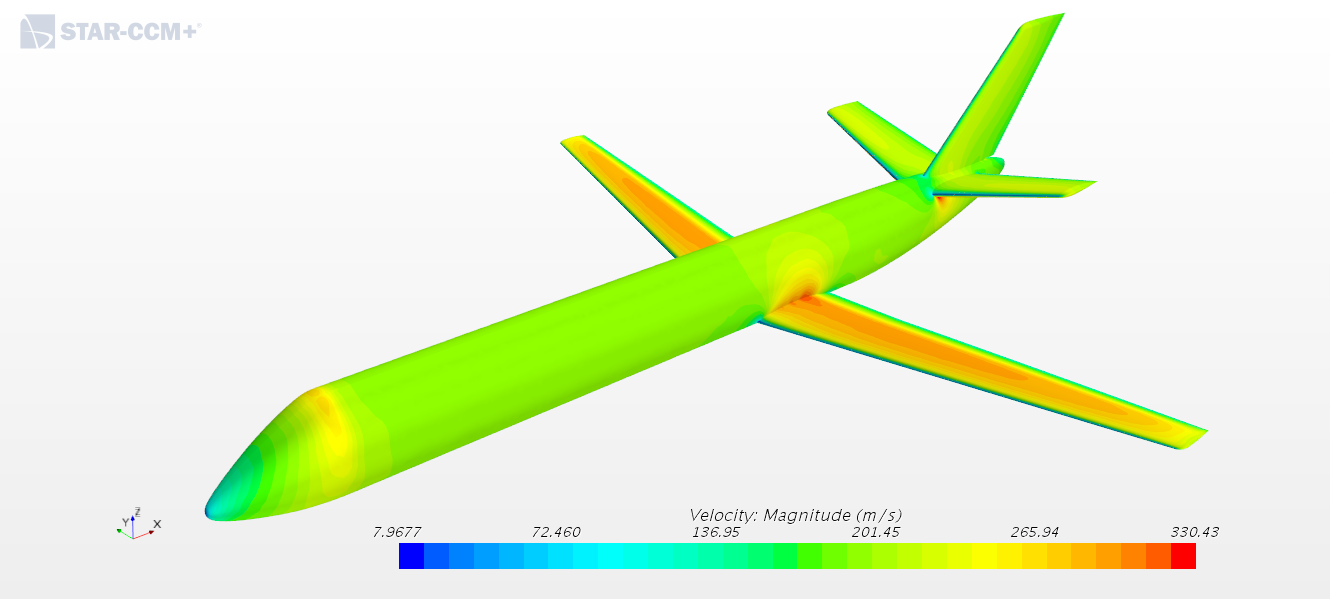
\includegraphics[scale=0.32]{Immagini/Capitolo4/Test_Sim_01_Scalar_Scene_1}
\caption{Velocity magnitude scalar scene for the no-canard configuration}
\label{fig:VMag_01}
\end{figure} 
%
\begin{figure}[H]
\centering
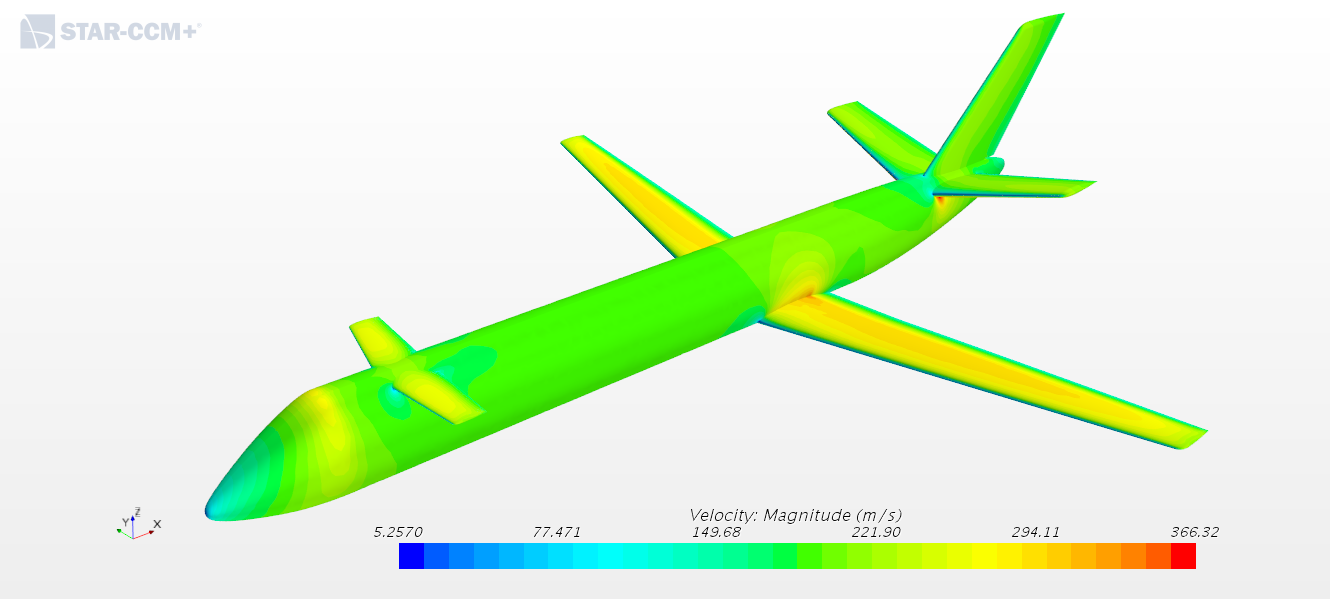
\includegraphics[scale=0.32]{Immagini/Capitolo4/Test_Sim_02_Scalar_Scene_1}
\caption{Velocity magnitude scalar scene for the canard-equipped configuration}
\label{fig:VMag_02}
\end{figure}  
%

